\pdfinfoomitdate=1
\pdftrailerid{}
\pdfsuppressptexinfo=15
\documentclass[11pt,openany]{report}
\usepackage[letterpaper,margin=0.82in,headheight=14pt]{geometry}
\usepackage[T1]{fontenc}
\usepackage[utf8]{inputenc}
\usepackage{lmodern}
\usepackage{microtype}
\usepackage{amsmath,amssymb,amsthm,mathtools}
\usepackage{booktabs,longtable,tabularx,array}
\usepackage{graphicx,float,placeins}
\usepackage{xcolor}
\usepackage{enumitem}
\usepackage{fancyhdr}
\usepackage{listings}
\usepackage[hidelinks]{hyperref}
\usepackage[nameinlink,noabbrev]{cleveref}
\usepackage{needspace}
\allowdisplaybreaks

\graphicspath{{figures/}}
\newcommand{\WalkRawPaths}{8191}
\newcommand{\WalkQuotientNodes}{25}
\newcommand{\WalkQuotientEdges}{46}
\newcommand{\AnalyticRawPaths}{315}
\newcommand{\AnalyticQuotientNodes}{77}
\newcommand{\AnalyticQuotientEdges}{149}
\newcommand{\PolynomialRawPaths}{781}
\newcommand{\PolynomialQuotientNodes}{224}
\newcommand{\PolynomialQuotientEdges}{355}
\newcommand{\SequenceRawPaths}{156}
\newcommand{\SequenceQuotientNodes}{111}
\newcommand{\SequenceQuotientEdges}{135}
\newcommand{\GaussianRawPaths}{2125}
\newcommand{\GaussianQuotientNodes}{126}
\newcommand{\GaussianQuotientEdges}{335}
\newcommand{\QubitRawPaths}{1365}
\newcommand{\QubitQuotientNodes}{6}
\newcommand{\QubitQuotientEdges}{24}
\newcommand{\MatrixRawPaths}{400}
\newcommand{\MatrixQuotientNodes}{55}
\newcommand{\MatrixQuotientEdges}{161}
\newcommand{\ShapeRawPaths}{259}
\newcommand{\ShapeQuotientNodes}{147}
\newcommand{\ShapeQuotientEdges}{210}
\newcommand{\GraphRawPaths}{150}
\newcommand{\GraphQuotientNodes}{17}
\newcommand{\GraphQuotientEdges}{41}
\newcommand{\AdicSimpleRawPaths}{10}
\newcommand{\AdicSimpleQuotientNodes}{10}
\newcommand{\AdicSimpleQuotientEdges}{8}
\newcommand{\AdicSingularRawPaths}{21}
\newcommand{\AdicSingularQuotientNodes}{21}
\newcommand{\AdicSingularQuotientEdges}{20}
\newcommand{\BuiltInChecks}{18}
\newcommand{\TestCount}{50}
\newcommand{\FigureCount}{20}
\newcommand{\ExampleCount}{11}


\hypersetup{
  pdftitle={Universal Generative Deformation Calculus: Visual Atlas and Worked Examples},
  pdfauthor={Komorebi P.},
  pdfsubject={Infinite perturbation forests, path quotients, branch completion, and family discovery}
}

\pagestyle{fancy}
\fancyhf{}
\fancyhead[L]{\small UGDC: Visual Atlas and Worked Examples}
\fancyhead[R]{\small Komorebi P.}
\fancyfoot[C]{\thepage}
\renewcommand{\headrulewidth}{0.4pt}

\setlength{\parindent}{0pt}
\setlength{\parskip}{0.55em}
\raggedbottom

\newtheorem{theorem}{Theorem}[chapter]
\newtheorem{proposition}[theorem]{Proposition}
\newtheorem{lemma}[theorem]{Lemma}
\newtheorem{corollary}[theorem]{Corollary}
\newtheorem{conjecture}[theorem]{Conjecture}
\theoremstyle{definition}
\newtheorem{definition}[theorem]{Definition}
\newtheorem{example}[theorem]{Worked example}
\newtheorem{algorithm}[theorem]{Algorithm}
\theoremstyle{remark}
\newtheorem{remark}[theorem]{Remark}
\newtheorem{boundary}[theorem]{Boundary statement}

\newcolumntype{L}[1]{>{\raggedright\arraybackslash}p{#1}}
\newcommand{\C}{\mathbb C}
\newcommand{\R}{\mathbb R}
\newcommand{\N}{\mathbb N}
\newcommand{\Z}{\mathbb Z}
\newcommand{\Tcal}{\mathcal T}
\newcommand{\Dcal}{\mathcal D}
\newcommand{\Ocal}{\mathcal O}
\newcommand{\Fcal}{\mathcal F}
\newcommand{\Pcal}{\mathcal P}
\newcommand{\Gcal}{\mathcal G}
\newcommand{\Xcal}{\mathcal X}
\newcommand{\Ecal}{\mathcal E}
\newcommand{\Path}{\operatorname{Path}}
\newcommand{\End}{\operatorname{End}}
\newcommand{\cost}{\operatorname{cost}}
\newcommand{\depth}{\operatorname{depth}}
\newcommand{\ev}{\operatorname{ev}}
\newcommand{\Reach}{\operatorname{Reach}}
\newcommand{\Inv}{\operatorname{Inv}}
\newcommand{\cl}{\operatorname{cl}}
\newcommand{\id}{\mathrm{id}}
\newcommand{\dd}{\,\mathrm d}
\newcommand{\norm}[1]{\left\lVert #1\right\rVert}
\newcommand{\abs}[1]{\left\lvert #1\right\rvert}

\lstset{
  basicstyle=\ttfamily\footnotesize,
  breaklines=true,
  frame=single,
  showstringspaces=false,
  columns=fullflexible,
  keepspaces=true
}

\title{\textbf{Universal Generative Deformation Calculus}\\[0.42em]
\large Visual Atlas and Worked Examples Edition\\[0.30em]
\normalsize Infinite Perturbation Forests, Path Quotients, Branch Completion, and Certified Family Discovery}
\author{Komorebi P.}
\date{August 2026\\Version 1.1.0}

\begin{document}
\maketitle

\begin{abstract}
A deformable object does not produce one neighboring object. It produces a direction space, and every resulting object carries a new direction space of its own. Repeating this rule creates an infinite tree of perturbations of perturbations. This paper makes that construction precise. The raw object is a typed path forest whose vertices are finite admissible routes. Relations identify routes with equivalent endpoints, giving a quotient deformation graph. A declared topology then adds limits of convergent infinite branches. Continuous direction spaces are handled by certified finite covers with propagated error bounds. Multi-input deformations replace the ordinary tree by an operadic hyperforest. Projectors on route cylinders give exact refinement and transfer identities. Growth entropy and weighted path zeta functions separate formal path complexity from genuinely distinct object complexity. A family certificate distinguishes repeated rediscovery from a parameterized family with proved closure laws. This visual-atlas edition adds twenty Python-generated figure pairs and eleven finite realizations. The examples cover integer routes, polynomial and analytic operators, sequence transforms, Gaussian probability laws, matrix operations, affine geometry, unlabeled graphs, projective qubits, congruence lifting, branch completion, and associative multi-input products. Every example records raw routes, quotient objects, failed operations, invariants, and reproducible tests.
\end{abstract}

\begin{center}
\fbox{\begin{minipage}{0.92\textwidth}
\textbf{Status.} The finite and analytic statements are proved under the hypotheses printed below. The software verifies the declared finite examples through \BuiltInChecks\ built-in checks and \TestCount\ independent tests. Every displayed figure is generated by the accompanying Python source. The phrase ``every direction'' always means every direction in a fixed admissible grammar. It does not mean every imaginable target-dependent map. Historical priority and external novelty are separate questions and are not asserted by this manuscript.
\end{minipage}}
\end{center}

\tableofcontents
\listoffigures
\listoftables
\clearpage

\chapter{The object being constructed}

\section{The central idea}

Fix an object $x_0$. At $x_0$ there is a collection of admissible abstract directions. Applying one direction gives a child object. The child is not forced to inherit the same direction list. It is queried again, and its own admissible directions create the next generation. This process continues without a preset depth.

The word direction is intentionally broad. It may mean a tangent vector, a parameter change, a differential operator, a rewrite, a projection, an inversion, a quotient, a coordinate transport, a physical interaction, a refinement, or a functorial move. What matters is that the direction belongs to a grammar declared before the target object is known.

There are three mathematical layers.

\begin{enumerate}[label=(\arabic*)]
\item The \emph{raw path forest} remembers every finite sequence of choices.
\item The \emph{quotient object graph} identifies paths that represent the same object or the same object up to a declared symmetry.
\item The \emph{completed boundary} adds limits represented by infinite compatible routes.
\end{enumerate}

Confusing these layers causes two opposite errors. Counting paths as objects exaggerates discovery because many routes may collapse to one endpoint. Keeping only endpoints loses construction history, multiplicity, and interference between routes.

\begin{figure}[H]
\centering
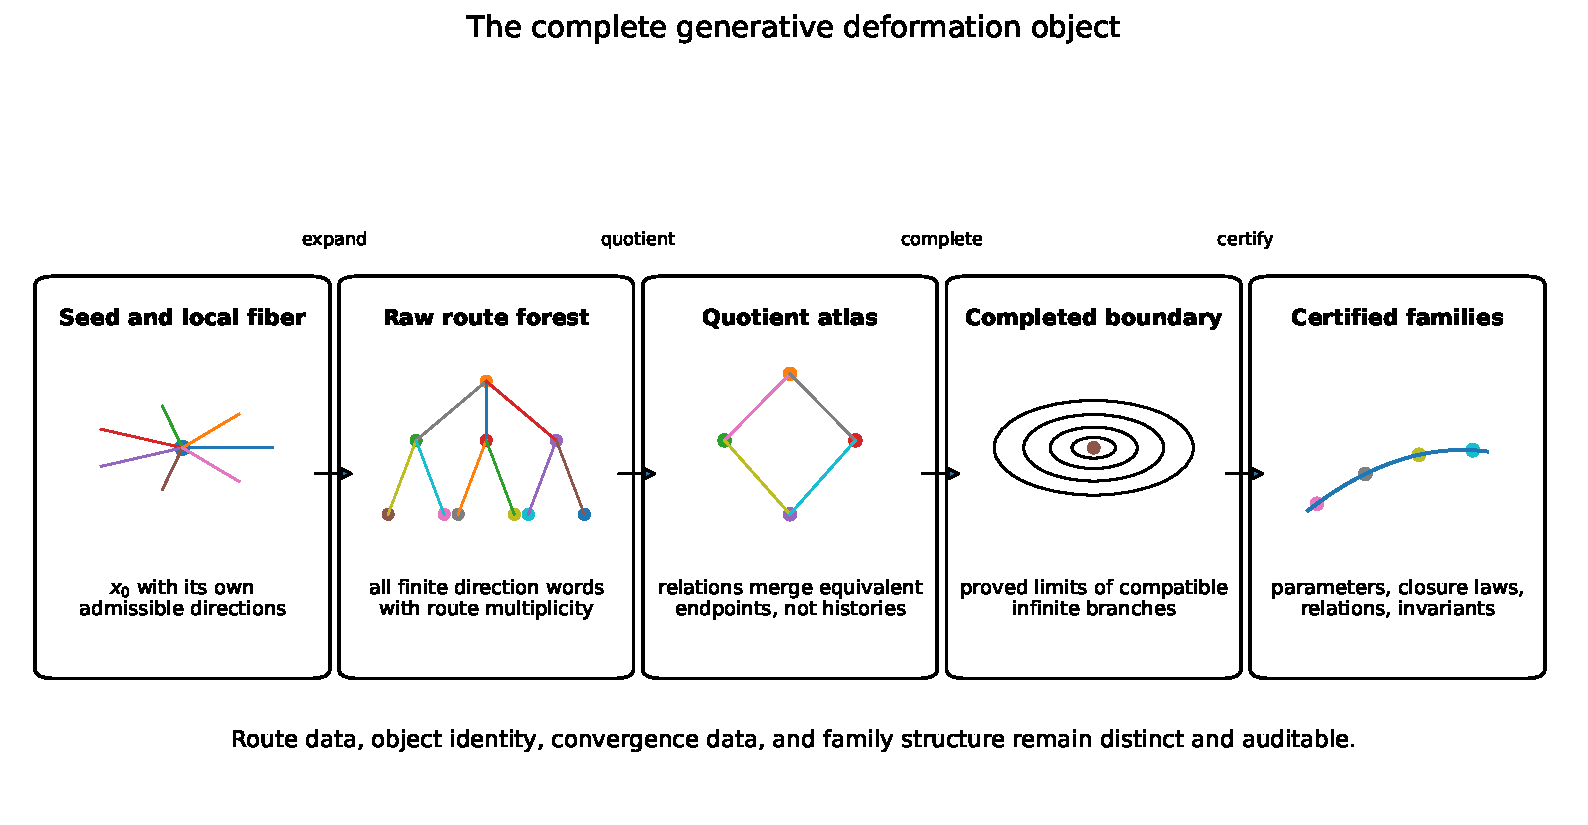
\includegraphics[width=0.98\textwidth]{00_universal_overview.pdf}
\caption{The complete object retains five distinct layers: a seed and its local direction fiber, the raw route forest, the relation quotient, the completed boundary, and certified families inside the completed universe.}
\label{fig:three-layers}
\end{figure}

\section{Why a fixed direction grammar is necessary}

Given any two objects $x$ and $y$, one can invent a one-step map that sends $x$ to $y$. Such a map does not reveal a generative structure. It hides the target inside the operation.

A meaningful construction therefore fixes the allowed direction rule before exploration begins. The grammar may be large, parameterized, or typed. It may even be countably infinite. It must still be independent of the particular endpoint one later hopes to find.

\begin{definition}[Anti-encoding condition]
A deformation grammar satisfies the anti-encoding condition when the following data are declared independently of the target endpoint:
\begin{enumerate}[label=(\alph*)]
\item the object types
\item the admissible direction fibers
\item the evaluation rules
\item the path relations and symmetries
\item the topology or completion rule
\item the cost and validity rules used by the explorer
\end{enumerate}
\end{definition}

The condition does not require every domain to use the same operations. It requires every claim of generation to name the operations that made generation possible.

\chapter{Typed deformation data}

\section{State-dependent direction fibers}

Let $\mathsf T$ be a set of types and let
\[
\Xcal=\coprod_{t\in\mathsf T}X_t
\]
be the disjoint union of the corresponding object spaces.

\begin{definition}[Direction bundle]
A direction bundle over $\Xcal$ is a map
\[
\pi:\Dcal\longrightarrow\Xcal.
\]
The fiber
\[
\Dcal_x=\pi^{-1}(x)
\]
is the complete set of directions admitted by the declared grammar at $x$.
\end{definition}

\begin{definition}[Elementary deformation law]
An elementary deformation law is a map
\[
\Phi:\Dcal\longrightarrow\Xcal
\]
with the understanding that $d\in\Dcal_x$ starts at $x$ and ends at $\Phi(d)$. We also write
\[
x\star d=\Phi(d).
\]
\end{definition}

The fiber $\Dcal_x$ may depend on every property of $x$. A matrix near a spectral collision may expose different directions from a diagonal matrix. A function with zeros may forbid reciprocal deformation. A singular algebraic point may have a larger tangent cone than a smooth point.

\begin{figure}[H]
\centering
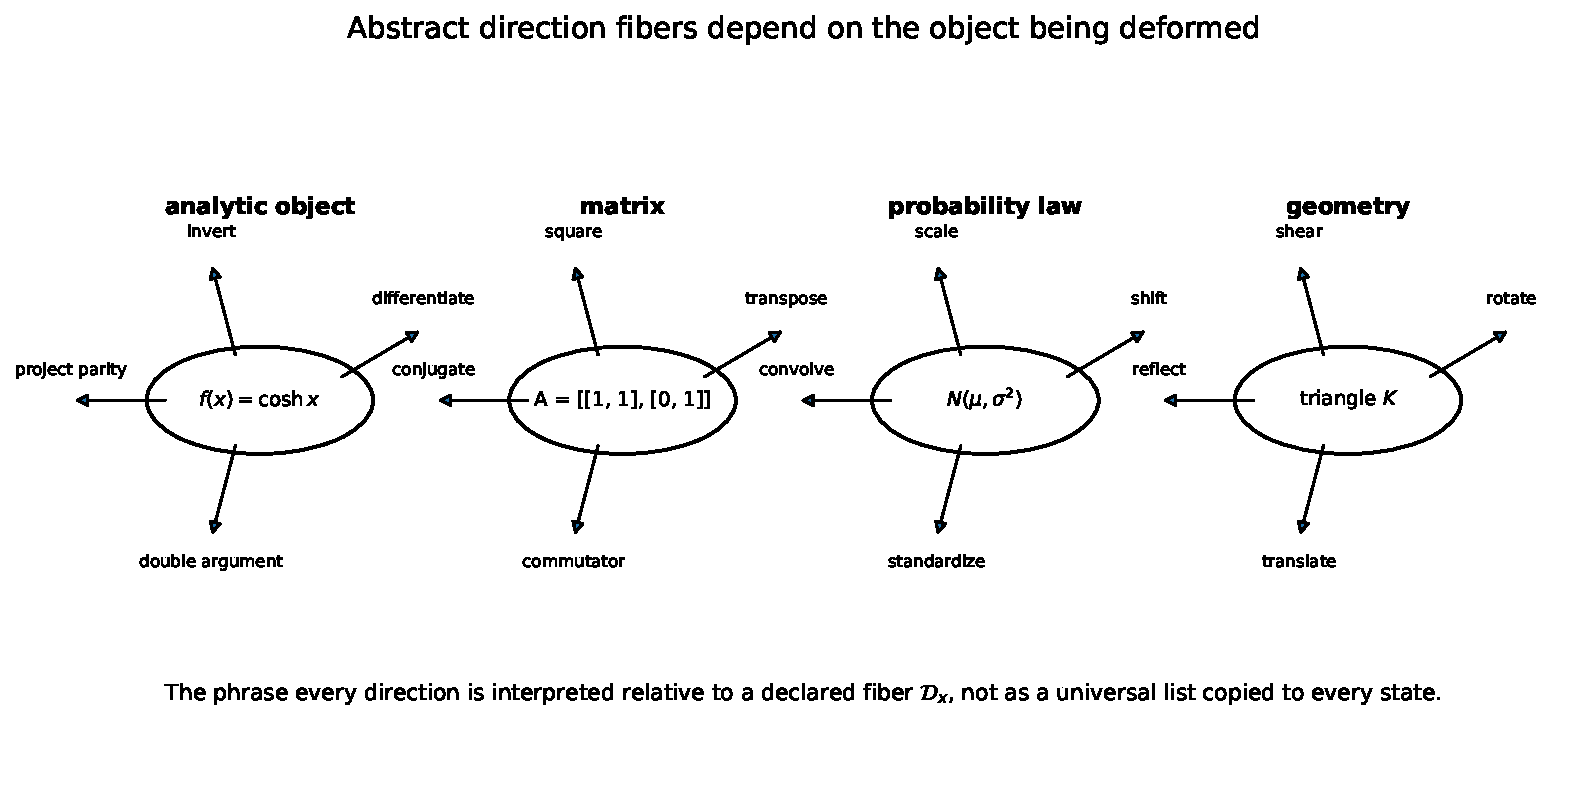
\includegraphics[width=0.98\textwidth]{01_direction_fiber_gallery.pdf}
\caption{A geometric direction bundle in action. Each deformed shape is queried again and can expose directions that were not useful or admissible at the root.}
\label{fig:direction-fibers}
\end{figure}

\begin{definition}[Typed generative deformation datum]
A typed generative deformation datum is a tuple
\[
\boxed{
\Gcal=
(\mathsf T,\Xcal,\pi:\Dcal\to\Xcal,\Phi,\mathcal R,\tau,\kappa,\mathcal V),
}
\]
where $\mathcal R$ is a path relation system, $\tau$ is a completion structure, $\kappa:\Dcal\to[0,\infty)$ is a direction cost, and $\mathcal V$ is a validity predicate.
\end{definition}

The data separate existence from computation. The full fiber $\Dcal_x$ defines the mathematics. A finite explorer may inspect only a subset, a finite cover, or a best-first frontier.

\section{Direction completeness}

\begin{definition}[Direction-complete expansion]
An expansion rule is direction-complete relative to $\Gcal$ at $x$ when it exposes every element of $\Dcal_x$. It is direction-complete through depth $n$ when this holds at every endpoint of every admissible path of length less than $n$.
\end{definition}

For a finite fiber, direction completeness is literal enumeration. For a countable fiber, it is fair lazy enumeration. For a continuous fiber, it is represented through parameter families and convergent covers. These cases must not be treated as if they were the same finite loop.

\chapter{The raw perturbation forest}

\section{Finite paths}

Fix a root $x_0\in\Xcal$.

\begin{definition}[Admissible path]
An admissible path of length $n$ from $x_0$ is a sequence
\[
\gamma=(d_1,\ldots,d_n)
\]
for which
\[
x_k=x_{k-1}\star d_k,
\qquad
d_k\in\Dcal_{x_{k-1}},
\qquad
1\le k\le n.
\]
Its endpoint is $\ev(\gamma)=x_n$. The empty path $\varnothing$ has endpoint $x_0$.
\end{definition}

Write $\Tcal_n(x_0)$ for the set of length-$n$ paths and
\[
\Tcal_{\mathrm{fin}}(x_0)=\coprod_{n\ge0}\Tcal_n(x_0).
\]
Every nonempty path has a unique parent obtained by deleting its final direction. Therefore $\Tcal_{\mathrm{fin}}(x_0)$ is a rooted tree even when different paths have the same endpoint.

\begin{theorem}[Exact reachability by depth]
For every $n\ge0$,
\[
\ev(\Tcal_n(x_0))
=
\Reach_n(x_0),
\]
where $\Reach_n(x_0)$ is the set obtained by applying exactly $n$ successive admissible directions.
\end{theorem}

\begin{proof}
The statement is immediate at depth zero. Assume it holds at depth $n$. Every path of length $n+1$ is a path of length $n$ followed by one direction from the fiber over its endpoint. Thus its endpoint lies in the $(n+1)$-step reachable set. Conversely, every object in the $(n+1)$-step reachable set is produced by an $n$-step reachable object and one admissible direction. The induction closes.
\end{proof}

\section{Universal property of the raw tree}

The raw tree is free in the precise sense that it imposes no relation beyond admissibility.

\begin{theorem}[Free rooted path property]
Let $Y$ be a rooted directed graph with root $y_0$. Suppose each admissible pair $(x,d)$ is assigned an edge operation on $Y$ in a way that depends only on the current image vertex and the label $d$. Then there is a unique root-preserving map
\[
F:\Tcal_{\mathrm{fin}}(x_0)\longrightarrow Y
\]
that follows those assigned edges along every path.
\end{theorem}

\begin{proof}
Set $F(\varnothing)=y_0$. If $F(\gamma)$ has been defined and $d$ is admissible at $\ev(\gamma)$, define $F(\gamma d)$ by following the assigned $d$-edge from $F(\gamma)$. Every path has one parent, so the definition is unambiguous. Any root-preserving map with the required edge behavior must obey the same recursion, which proves uniqueness.
\end{proof}

This theorem is simple, but it fixes the object correctly. The tree stores construction histories before any identities are imposed.

\section{Costs and path metadata}

The cost of a finite path is
\[
\cost(\gamma)=\sum_{k=1}^n\kappa(d_k).
\]
A path record may also store error bounds, provenance, validity certificates, symbolic assumptions, and the first place at which an invariant changed. None of these fields alters reachability. They determine how a finite explorer prioritizes and audits the infinite object.

\chapter{Relations and the quotient deformation graph}

\section{Path congruence}

Two different paths may represent the same endpoint. They may also represent endpoints related by a symmetry that the domain regards as immaterial.

\begin{definition}[Extension-compatible path relation]
An equivalence relation $\sim$ on finite paths is extension-compatible when the following implication holds. If $\gamma\sim\eta$ and a direction label $d$ is admissible after both paths with compatible meaning, then
\[
\gamma d\sim\eta d.
\]
The relation may also identify endpoints under a declared symmetry group, rewrite system, canonical form, gauge, or quotient law.
\end{definition}

\begin{definition}[Quotient deformation graph]
The quotient deformation graph is
\[
\boxed{
\Ocal(x_0)=\Tcal_{\mathrm{fin}}(x_0)/\sim.
}
\]
Its vertices are relation classes of paths. An edge is induced by one admissible extension.
\end{definition}

\begin{theorem}[Well-defined quotient extension]
If $\sim$ is extension-compatible, then the edge induced by an admissible direction does not depend on the representative of a path class.
\end{theorem}

\begin{proof}
Choose representatives $\gamma$ and $\eta$ of one class. By extension compatibility, every common admissible extension satisfies $\gamma d\sim\eta d$. Therefore both representatives determine the same child class.
\end{proof}

The quotient need not remain a tree. Relations can create merges and cycles. The correct object is generally a directed graph, a category, or a groupoid.

\section{Canonical keys and exact deduplication}

A computational realization uses a canonical key
\[
K:\Xcal\longrightarrow\mathcal K
\]
with
\[
K(x)=K(y)
\quad\Longleftrightarrow\quad
x\sim y
\]
for the declared finite example. Exact polynomial coefficients, reduced rational numbers, canonical symbolic expressions, and normalized matrices are suitable examples. Floating point rounding alone is not an exact quotient relation.

\begin{boundary}[Canonicalization boundary]
A finite program can certify the quotient only to the strength of its canonicalizer. A key collision that is not a mathematical equivalence destroys soundness. A failure to identify equivalent objects preserves soundness but overcounts quotient vertices.
\end{boundary}

\section{Exact example: the integer walk}

Let the root be $0\in\Z$. Every integer has two directions,
\[
+1,
\qquad
-1.
\]
A path of length $n$ is a word in these two labels.

\begin{theorem}[Raw and quotient growth of the integer walk]
At exact depth $n$, the raw path count is $2^n$. The distinct endpoint count is $n+1$.
\end{theorem}

\begin{proof}
There are two choices at every step, giving $2^n$ words. If a path contains $k$ negative steps, its endpoint is
\[
(n-k)-k=n-2k.
\]
As $k$ ranges from $0$ to $n$, these are $n+1$ distinct integers. Every path with the same value of $k$ has the same endpoint.
\end{proof}

\begin{table}[htbp]
\centering
\caption{Raw paths and distinct quotient endpoints for the integer walk.}
\label{tab:walk-growth}
\begin{tabular}{rrr}
\toprule
Depth & Raw paths & Distinct endpoints \\
\midrule
0 & 1 & 1 \\
1 & 2 & 2 \\
2 & 4 & 3 \\
3 & 8 & 4 \\
4 & 16 & 5 \\
5 & 32 & 6 \\
6 & 64 & 7 \\
7 & 128 & 8 \\
8 & 256 & 9 \\
9 & 512 & 10 \\
10 & 1024 & 11 \\
11 & 2048 & 12 \\
12 & 4096 & 13 \\
\bottomrule
\end{tabular}
\end{table}


\begin{figure}[H]
\centering
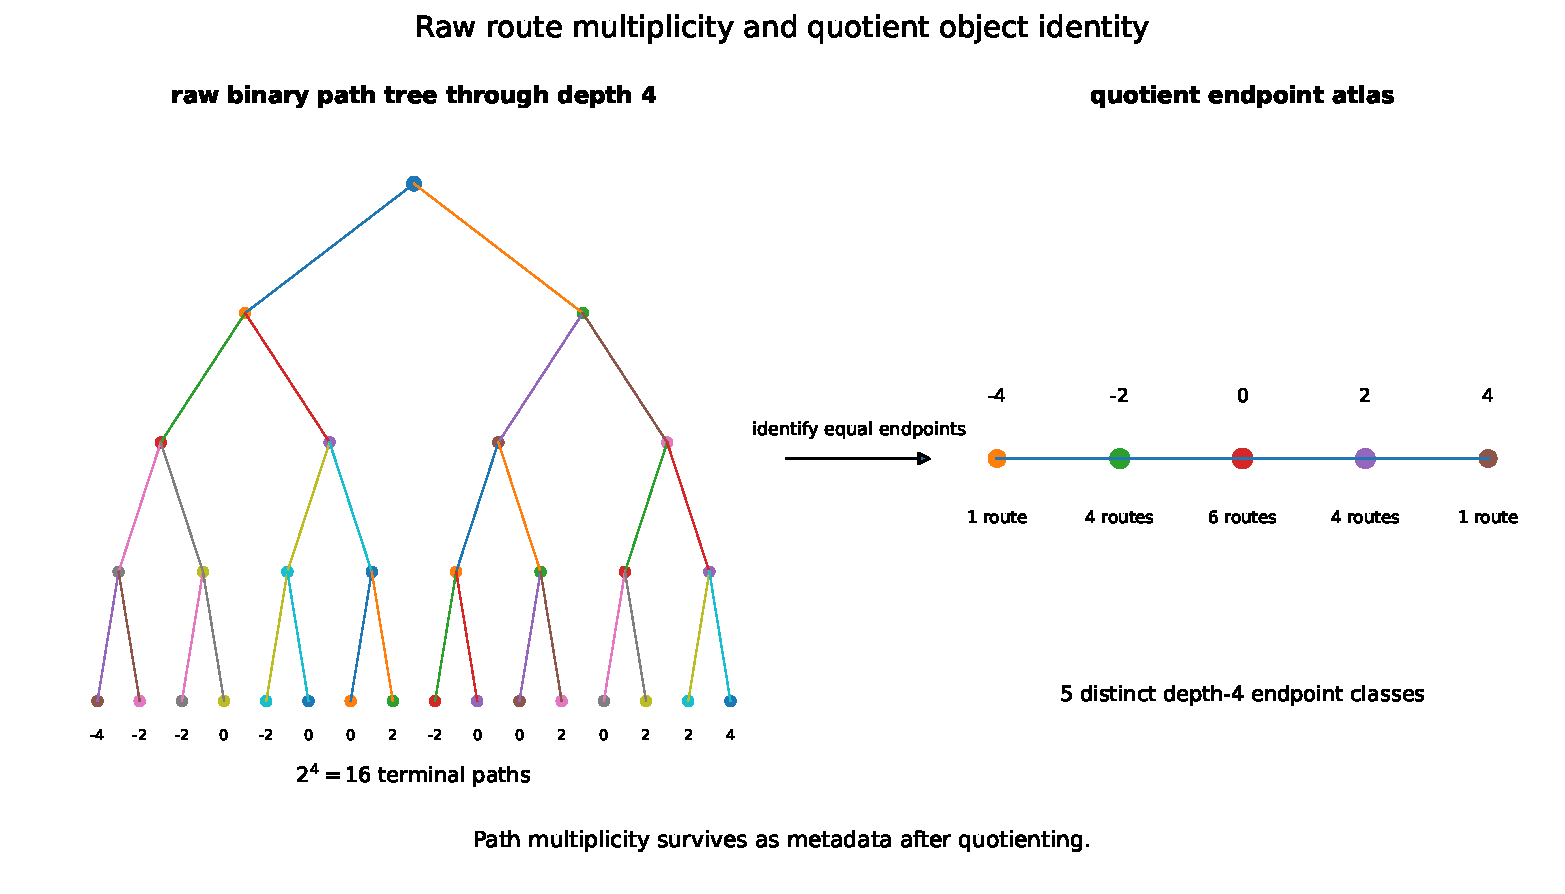
\includegraphics[width=0.98\textwidth]{02_raw_tree_to_quotient.pdf}
\caption{A finite route tree and its quotient graph are shown side by side. Repeated endpoints merge, while route multiplicities and the path archive remain available.}
\label{fig:raw-quotient}
\end{figure}

This example shows why the word tree must be used carefully. The path object is a binary tree. The object quotient is a line with repeated directed traffic.

\chapter{Continuous direction spaces}

\section{Why literal enumeration is impossible}

A tangent sphere, a parameter interval, or a cone of admissible perturbations may be uncountable. No finite or countable loop can visit every real parameter individually. The correct representation keeps the direction family as one mathematical object and explores it through finite covers.

Let each fiber $\Dcal_x$ carry a metric $\rho_x$. A finite set $N_\epsilon(x)\subseteq\Dcal_x$ is an $\epsilon$-net when every $d\in\Dcal_x$ lies within $\epsilon$ of some $\widehat d\in N_\epsilon(x)$.

\section{Propagated cover theorem}

Assume the object space carries a metric $d_X$.

\begin{theorem}[Pathwise cover error]
Consider an exact route
\[
x_k=x_{k-1}\star d_k
\]
and a sampled route
\[
\widehat x_k=\widehat x_{k-1}\star\widehat d_k.
\]
Suppose at step $k$,
\[
d_X(x\star d,y\star e)
\le
L_k d_X(x,y)+M_k\rho(d,e),
\]
and
\[
\rho(d_k,\widehat d_k)\le\epsilon_k.
\]
Then
\[
\boxed{
 d_X(x_n,\widehat x_n)
 \le
 \left(\prod_{k=1}^nL_k\right)d_X(x_0,\widehat x_0)
 +
 \sum_{j=1}^n
 M_j\epsilon_j
 \prod_{k=j+1}^nL_k.
}
\]
\end{theorem}

\begin{proof}
Set $e_k=d_X(x_k,\widehat x_k)$. The hypothesis gives
\[
e_k\le L_ke_{k-1}+M_k\epsilon_k.
\]
Repeated substitution yields the displayed formula.
\end{proof}

\begin{corollary}[Convergent direction covers]
If $L_k\le1$, $M_k\le M$, and
\[
\sum_{k\ge1}\epsilon_k<\infty,
\]
then the total endpoint error of the sampled route is bounded uniformly in depth by
\[
M\sum_{k\ge1}\epsilon_k
\]
when the roots coincide.
\end{corollary}

\begin{figure}[H]
\centering
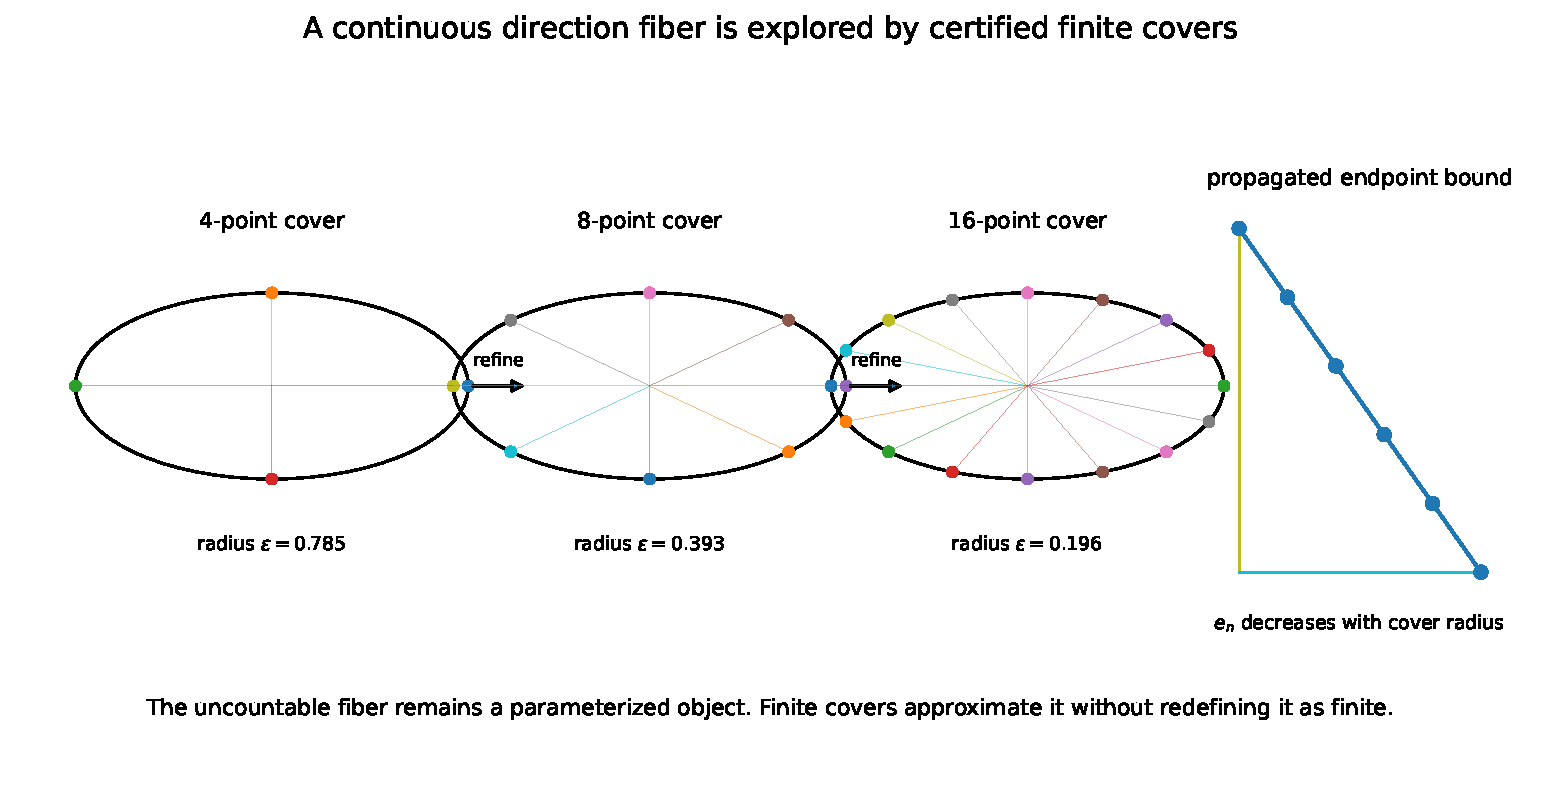
\includegraphics[width=0.98\textwidth]{03_continuous_direction_covers.pdf}
\caption{A continuous direction family is approximated by nested finite covers. The right panel records the certified geometric decrease of the direction-cover radius.}
\label{fig:cover-error}
\end{figure}

\section{Parameterized edges rather than sampled edges}

Sampling is an execution method, not the definition of the continuous forest. A continuous family is stored symbolically as an edge bundle
\[
\Ecal_x
=
\{(d,x\star d):d\in\Dcal_x\}.
\]
Finite nets approximate this bundle. Refinement replaces one coarse parameter cell by smaller cells. The cell itself remains a first-class object with a radius and a coverage certificate.

\chapter{Infinite branches and completion}

\section{The boundary of the raw forest}

An infinite route is a sequence
\[
\omega=(d_1,d_2,\ldots)
\]
whose every finite prefix is admissible. The set of infinite routes is the path boundary $\partial\Tcal(x_0)$.

An infinite route does not automatically determine an object of $\Xcal$. A topology, metric, inverse limit, direct limit, or weak convergence rule is required.

\begin{definition}[Convergent route]
A route $\omega$ is convergent in a metric realization when its endpoint sequence
\[
x_0,x_1,x_2,\ldots
\]
converges in the declared completion $\widehat\Xcal$.
\end{definition}

\begin{theorem}[Summable-step convergence]
Suppose $\widehat\Xcal$ is complete and
\[
d_X(x_{n+1},x_n)\le a_n
\]
with
\[
\sum_{n\ge0}a_n<\infty.
\]
Then $(x_n)$ is Cauchy and the route has a unique limit in $\widehat\Xcal$.
\end{theorem}

\begin{proof}
For $m>n$,
\[
d_X(x_m,x_n)
\le
\sum_{k=n}^{m-1}d_X(x_{k+1},x_k)
\le
\sum_{k=n}^{m-1}a_k.
\]
The tail tends to zero. Completeness supplies a unique limit.
\end{proof}

\section{Dyadic route example}

Starting at $0$, let the directions at depth $n$ be
\[
\pm2^{-(n+1)}.
\]
Every infinite sign route converges because
\[
\sum_{n\ge0}2^{-(n+1)}=1.
\]
The boundary therefore maps into $[-1,1]$. Different sign sequences can represent the same endpoint only at the usual binary-expansion ambiguity, which can be handled by a path relation.

\begin{figure}[H]
\centering
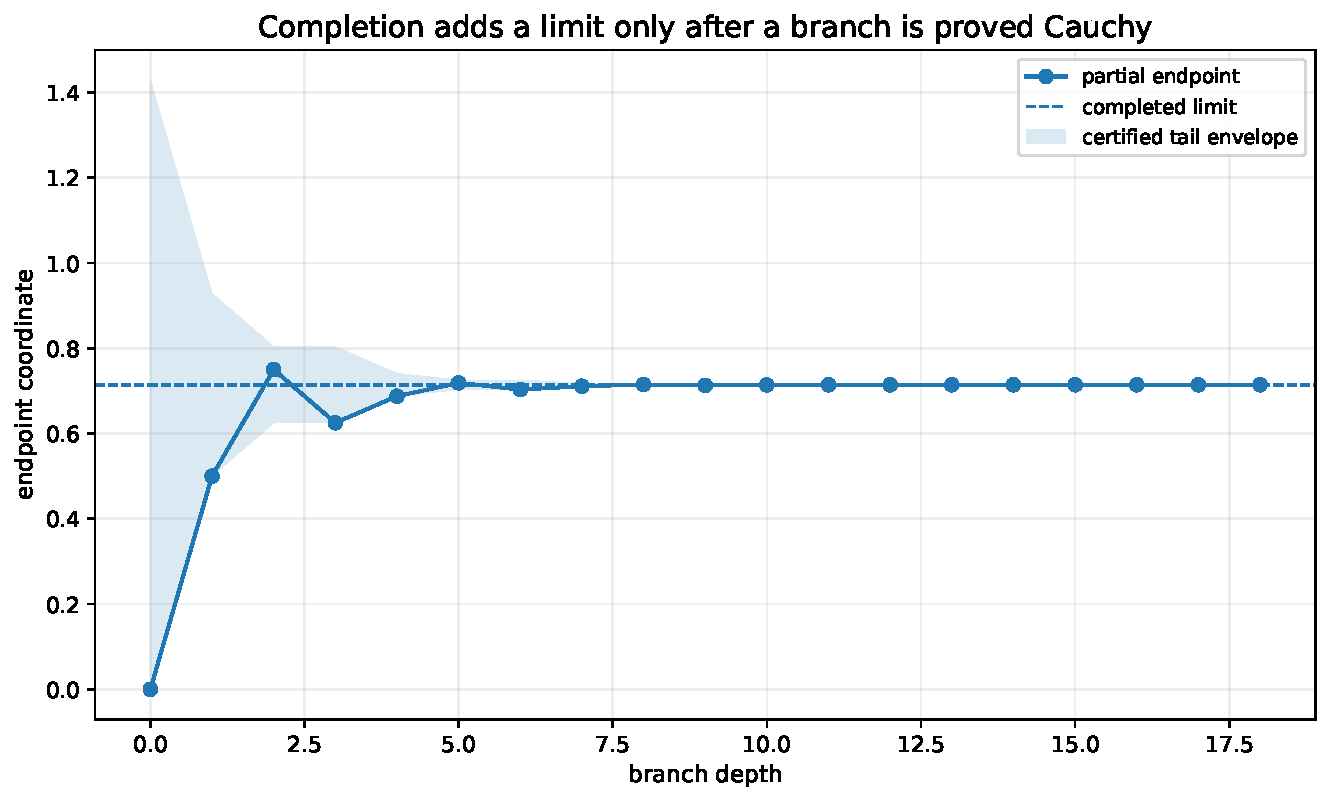
\includegraphics[width=0.98\textwidth]{04_branch_completion.pdf}
\caption{A summable perturbation branch converges inside the declared completion. Finite prefixes, tail bounds, and the limiting object remain separate parts of the certificate.}
\label{fig:branch-convergence}
\end{figure}

\section{Inverse and direct limits}

Metric completion is not the only possibility. In arithmetic deformation, a branch may be a compatible tower
\[
x_1\leftarrow x_2\leftarrow x_3\leftarrow\cdots
\]
whose object is an inverse limit. In nested function spaces, a branch may enter a direct limit. In weak probability or operator topologies, convergence may be defined only against a test class.

The calculus therefore treats completion as declared data. It never replaces one mode of convergence with another silently.

\chapter{Nonlinear and multi-input perturbations}

\section{Why unary routes are not enough}

Some directions combine several previously generated objects. Addition, multiplication, tensoring, composition, gluing, and nonlinear interaction are multi-input operations. Their natural combinatorial object is not an ordinary rooted path tree.

For every $r\ge2$, let
\[
\Psi_r:
\Xcal^r\times\Dcal^{(r)}
\longrightarrow
\Xcal
\]
be a typed $r$-input deformation law.

\begin{definition}[Operadic perturbation hyperforest]
The operadic perturbation hyperforest generated by a seed family is the set of all finite rooted typed trees whose leaves are seeds and whose internal vertices are labeled by admissible operations $\Phi$ or $\Psi_r$. Evaluation proceeds from leaves to root.
\end{definition}

\begin{figure}[H]
\centering
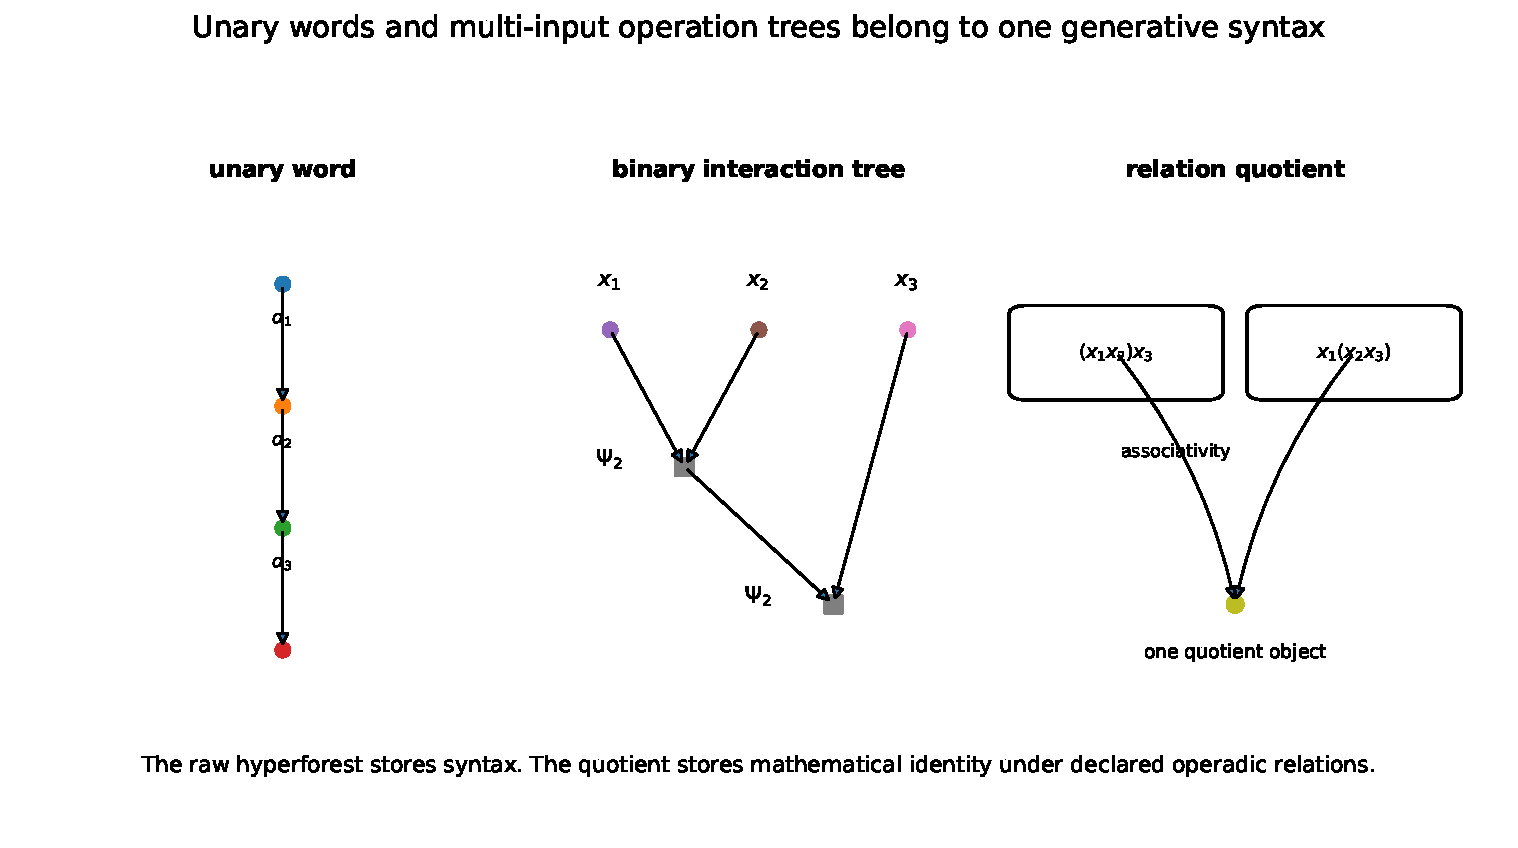
\includegraphics[width=0.98\textwidth]{05_operadic_hyperforest.pdf}
\caption{Unary routes and multi-input operations form different generative geometries. A binary product joins two parents, while an operadic hyperforest retains the complete input arity and syntax.}
\label{fig:operadic}
\end{figure}

\section{Free operadic property}

\begin{theorem}[Free interaction construction]
Before relations are imposed, every finite expression built from the declared seeds and multi-input operations has a unique rooted syntax tree. Any interpretation that assigns compatible concrete operations to the primitive labels extends uniquely to an evaluation of all such trees.
\end{theorem}

\begin{proof}
Every finite expression is parsed recursively into its outermost operation and its input expressions. This gives a rooted tree. Evaluation is defined from the leaves upward. Uniqueness follows because any compatible interpretation must evaluate each internal vertex by the operation written at that vertex.
\end{proof}

Relations such as associativity, commutativity, distributivity, gauge equivalence, and analytic identities then quotient the free syntax trees.

\section{Repeated quadratic substitution}

Consider
\[
u=s+\lambda u^2.
\]
Repeated substitution expands $u$ into rooted binary trees. If only shape is counted, the number of binary trees with $n$ internal vertices is the Catalan number $C_n$.

\begin{proposition}[Catalan interaction growth]
The counts satisfy
\[
C_0=1,
\qquad
C_{n+1}=\sum_{k=0}^nC_kC_{n-k}.
\]
\end{proposition}

\begin{proof}
At the root of a binary tree with $n+1$ internal vertices, the left subtree has $k$ internal vertices and the right subtree has $n-k$. Summing over all $k$ gives the recurrence.
\end{proof}

The first values are
\[
1,1,2,5,14,42,132,429,\ldots.
\]
The rapid growth is not an implementation defect. It is the intrinsic size of the free nonlinear syntax before identities, symmetries, truncation rules, or cost weights are applied.

\chapter{Projectors on the perturbation forest}

\section{Path Hilbert spaces}

For a finite or countable depth layer, define
\[
\mathcal H_n=\ell^2(\Tcal_n(x_0)).
\]
The canonical basis vector associated with a path $\gamma$ is written $\lvert\gamma\rangle$.

For a prefix $\alpha$ of length $k\le n$, define the cylinder projector
\[
P^{(n)}_\alpha
\lvert\gamma\rangle
=
\begin{cases}
\lvert\gamma\rangle,&\alpha\text{ is a prefix of }\gamma,\\
0,&\text{otherwise}.
\end{cases}
\]

\begin{theorem}[Exact cylinder refinement]
For every prefix $\alpha$ and every depth $n>\abs{\alpha}$,
\[
\boxed{
P^{(n)}_\alpha
=
\sum_{d\in\Dcal_{\ev(\alpha)}}P^{(n)}_{\alpha d},
}
\]
with strong convergence when the child set is countable.
\end{theorem}

\begin{proof}
The descendant cylinder of $\alpha$ is the disjoint union of the descendant cylinders of its one-step children. Orthogonal projection onto a disjoint union of basis supports is the sum of the corresponding orthogonal projectors.
\end{proof}

This identity is the exact packet refinement law for perturbation routes.

\section{Mixed-depth cuts}

A complete cut is a prefix-free set $\Gamma$ meeting every infinite route exactly once. Its projectors satisfy
\[
\sum_{\alpha\in\Gamma}P_\alpha=I.
\]
Thus one branch may be resolved deeply while another stops early. Adaptive exploration can be represented without discarding the unresolved region.

\section{Transfer blocks between route packets}

Let $A:\mathcal H\to\mathcal K$ be a bounded operator and let $\{P_\alpha\}$ and $\{Q_\beta\}$ be complete route resolutions. Define
\[
A_{\beta\alpha}=Q_\beta A P_\alpha.
\]
Then
\[
A=\sum_{\alpha,\beta}A_{\beta\alpha}.
\]
If $B$ follows $A$, then
\[
(BA)_{\gamma\alpha}
=
\sum_\beta B_{\gamma\beta}A_{\beta\alpha}.
\]
Every operator composition becomes a sum over compatible intermediate perturbation packets.

\chapter{Growth, entropy, and path zeta functions}

\section{Two growth sequences}

Define
\[
a_n=\#\Tcal_n(x_0)
\]
for raw paths and
\[
q_n=\#\bigl(\ev(\Tcal_n(x_0))/\sim\bigr)
\]
for distinct quotient endpoints at exact depth $n$.

The raw branching entropy and object entropy are
\[
h_{\mathrm{raw}}
=
\limsup_{n\to\infty}\frac1n\log a_n,
\qquad
h_{\mathrm{obj}}
=
\limsup_{n\to\infty}\frac1n\log q_n.
\]
Always
\[
h_{\mathrm{obj}}\le h_{\mathrm{raw}}.
\]
The gap measures how much formal construction redundancy is removed by identities and symmetries.

\section{Weighted partition function}

Define
\[
Z_{x_0}(s)
=
\sum_{\gamma\ne\varnothing}
\exp\bigl(-s\cost(\gamma)\bigr).
\]
This is a path partition function. It weights short, inexpensive routes more strongly than long, expensive routes.

\begin{theorem}[Geometric convergence bound]
Suppose every vertex has at most $B$ children and every direction costs at least $c>0$. Then
\[
Z_{x_0}(s)
\le
\sum_{n\ge1}B^ne^{-scn}.
\]
Consequently, $Z_{x_0}(s)$ converges whenever
\[
sc>\log B.
\]
In a full regular $B$-ary tree with constant cost $c$, it diverges whenever $sc\le\log B$.
\end{theorem}

\begin{proof}
There are at most $B^n$ paths of length $n$, and each has cost at least $cn$. The upper bound is a geometric series with ratio $Be^{-sc}$. In the regular constant-cost case, equality holds at every depth, giving the divergence statement.
\end{proof}

\begin{figure}[H]
\centering
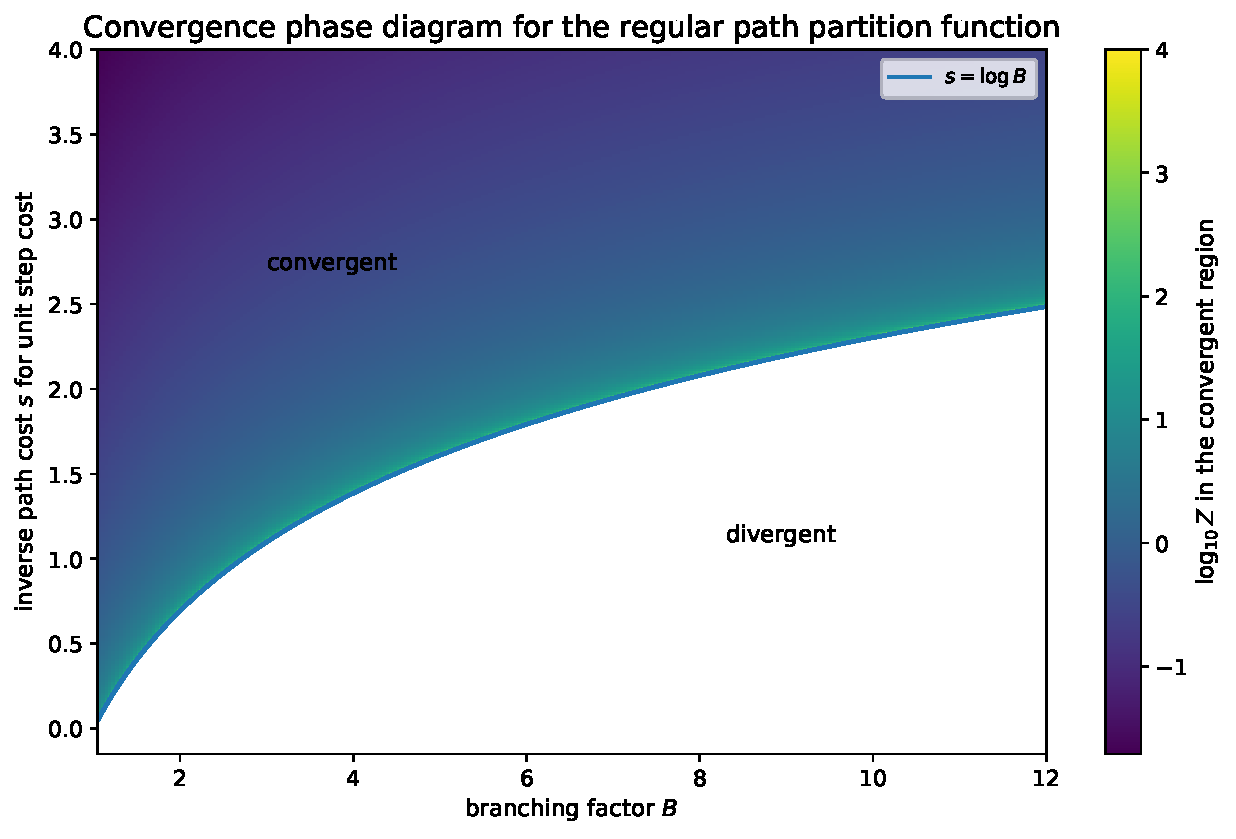
\includegraphics[width=0.98\textwidth]{06_growth_phase_diagram.pdf}
\caption{The regular-tree phase diagram separates convergent and divergent weighted path sums. Branching and route cost compete through the threshold $sc=\log B$.}
\label{fig:partition}
\end{figure}

\section{Why the quotient zeta function may be better}

A path zeta function measures construction complexity. A quotient zeta function measures distinct object complexity. Depending on the application, one may define
\[
Z_{\mathrm{obj}}(s)
=
\sum_{[x]\in\Ocal(x_0)}e^{-sC([x])},
\]
where $C([x])$ is the least path cost reaching the class. The two functions answer different questions and should be stored together.

\chapter{Certified discovery of mathematical families}

\section{From isolated endpoints to families}

An explorer may generate thousands of endpoints without discovering one coherent family. A family requires more than repeated resemblance.

\begin{definition}[Generated family certificate]
A generated family certificate is a tuple
\[
\Fcal=(\Theta,F,\{\sigma_d\}_{d\in A},\mathcal Q,\mathcal I),
\]
where
\begin{enumerate}[label=(\alph*)]
\item $\Theta$ is a parameter space
\item $F:\Theta\to\Ocal(x_0)$ assigns an object class to every parameter
\item $A$ is a collection of closure directions
\item $\sigma_d:\Theta\to\Theta$ satisfies
\[
F(\sigma_d(\theta))=d\cdot F(\theta)
\]
for every declared closure direction
\item $\mathcal Q$ is a set of exact relations or recurrences
\item $\mathcal I$ is a set of invariants shared or predictably transformed across the family
\end{enumerate}
\end{definition}

\begin{theorem}[Inductive soundness of a family certificate]
Suppose the seed member $F(\theta_0)$ is valid, every closure identity is proved, and every relation in $\mathcal Q$ is preserved by the parameter actions. Then every finite parameter word in the maps $\sigma_d$ produces a valid member of the certified family.
\end{theorem}

\begin{proof}
The root parameter gives a valid member. If a valid member has parameter $\theta$, applying a closure direction $d$ gives $F(\sigma_d(\theta))$ by the closure identity. The preserved relations remain true after the step. Induction over the parameter word proves the claim.
\end{proof}

\begin{figure}[H]
\centering
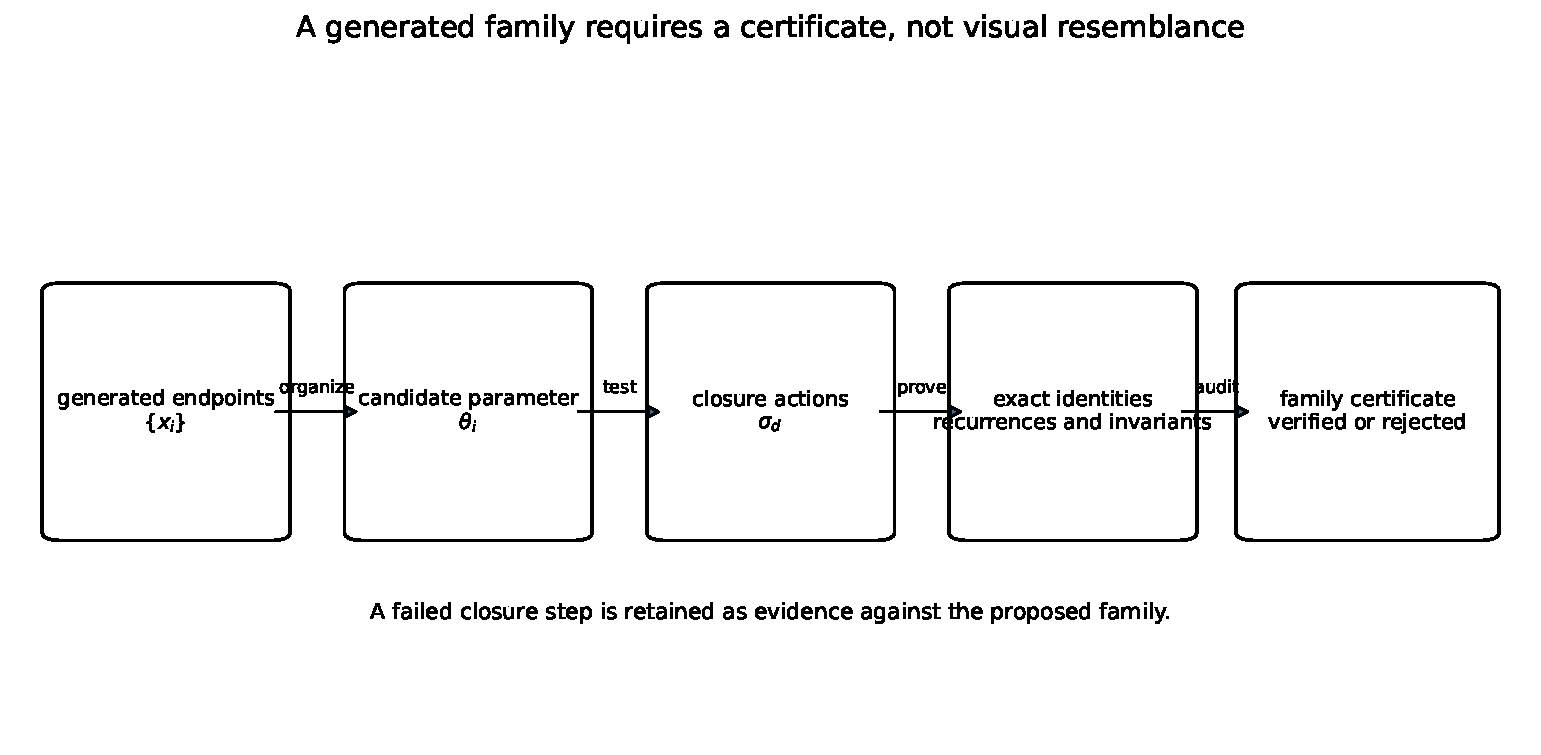
\includegraphics[width=0.99\textwidth]{07_family_certificate_pipeline.pdf}
\caption{Generated endpoints become a mathematical family only after a parameterization, closure actions, exact identities, recurrences, and invariants have been verified. Failed closure steps are retained as negative evidence.}
\label{fig:family-certificate}
\end{figure}

\section{Discovery is not historical novelty}

A family certificate proves internal structure. It does not prove that the family is absent from the literature. It also does not prove that two differently written certificates define different families. A separate comparison must check equivalence under reparameterization, analytic continuation, known transforms, and classical special cases.

\begin{boundary}[Novelty boundary]
The software uses the word discovery for a new relation or family relative to the explored archive and declared canonicalizers. It does not use finite computation as a certificate of historical priority.
\end{boundary}

\section{Recurrence certificates}

For a sequence $a_0,a_1,\ldots$, the implementation can search for a constant-coefficient relation
\[
a_n=c_1a_{n-1}+\cdots+c_ra_{n-r}
\]
using exact rational linear algebra. A proposed recurrence is accepted only when it reproduces every supplied term exactly. The built-in Fibonacci example recovers
\[
(c_1,c_2)=(1,1).
\]
This is a small example of the certificate principle. Fitting alone is not enough. The relation must be verified and then proved or bounded on the intended domain.

\chapter{Finite exploration of the infinite object}

\section{Breadth-first relation-reduced exploration}

The reference explorer stores raw paths and quotient nodes simultaneously.

\begin{algorithm}[Audited breadth-first exploration]
Given a deformation system, roots, a depth bound, and resource limits:
\begin{enumerate}[label=\arabic*.]
\item Insert each root as a raw path and a quotient node.
\item Remove the oldest path from the frontier.
\item Query the direction fiber of its endpoint.
\item Apply every exposed direction.
\item Validate the child and record failures explicitly.
\item Compute the canonical relation key.
\item Reuse an existing quotient node or create a new one.
\item Record the directed edge and its path multiplicity.
\item Insert the new raw path even when its endpoint was already known.
\item Repeat until the frontier, depth, or resource limit is exhausted.
\end{enumerate}
\end{algorithm}

Keeping the new path after endpoint deduplication is essential. It preserves the raw tree count and route multiplicity.

\begin{figure}[H]
\centering
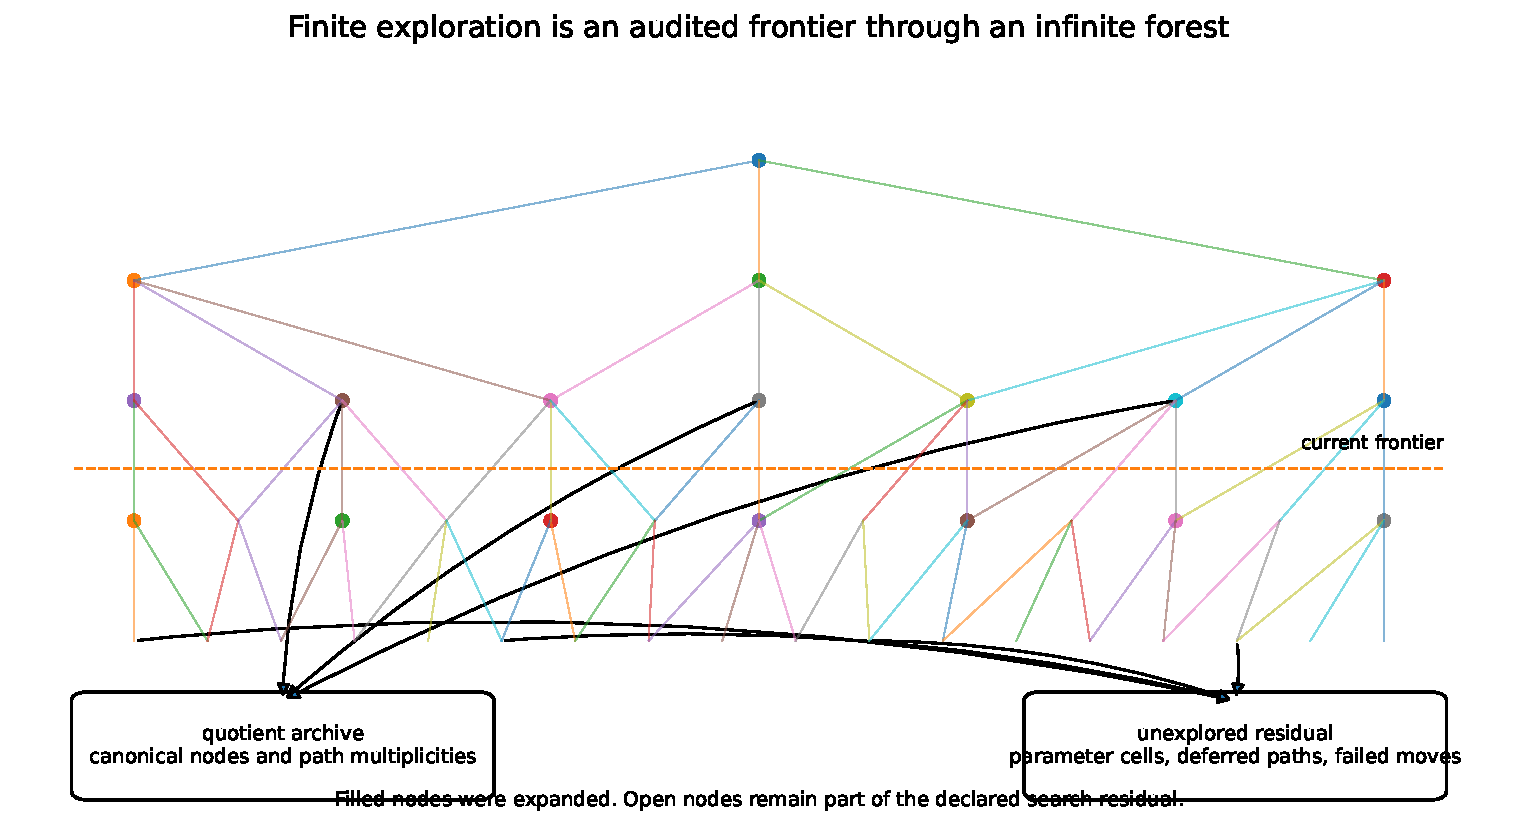
\includegraphics[width=0.99\textwidth]{08_exploration_frontier.pdf}
\caption{A finite computation is an audited frontier through an infinite forest. Expanded nodes, quotient nodes, deferred parameter cells, and failed moves are retained explicitly.}
\label{fig:pipeline}
\end{figure}

\begin{theorem}[Finite-depth completeness]
If every direction fiber reached before depth $N$ is finite and the breadth-first explorer has no active resource cap below the resulting path count, then it records every admissible path of length at most $N$.
\end{theorem}

\begin{proof}
Breadth-first exploration inserts every root. Assume every path of length $n<N$ is eventually removed from the frontier. The algorithm queries its complete finite direction fiber and inserts every one-step extension. Therefore every path of length $n+1$ is inserted. Induction proves the result.
\end{proof}

\section{Fair enumeration of countable fibers}

When a fiber is countably infinite, exhausting one vertex before visiting another may starve entire branches. A fair explorer dovetails local enumerators. For example, at global stage $m$ it may inspect the first $m$ directions of every path among the first $m$ frontier paths.

\begin{proposition}[Fairness consequence]
If every local countable fiber has a fixed enumeration and the global scheduler is fair, then every finite admissible path is eventually generated.
\end{proposition}

\begin{proof}
A finite path uses finitely many local direction indices. Fairness eventually reaches the required index at the root, then at the selected child, and so on through the finite route.
\end{proof}

\section{Best-first search and its limitation}

Cost-ordered search may reach useful objects much earlier than breadth-first search. It is not complete under an infinite budget unless the scheduling rule prevents starvation. A finite beam search is deliberately incomplete. Its output is a searched prefix plus an unexplored residual, not the entire forest.

\chapter{Stability of perturbations of perturbations}

\section{Two systems being compared}

Let $\Phi_k$ and $\widetilde\Phi_k$ be exact and perturbed deformation laws along corresponding routes. Suppose
\[
d_X(\Phi_k(x,d),\widetilde\Phi_k(y,e))
\le
L_kd_X(x,y)+M_k\rho(d,e)+\eta_k,
\]
where $\eta_k$ measures model error.

\begin{theorem}[Recursive deformation stability]
If the direction mismatch at step $k$ is at most $\epsilon_k$, then the endpoint error satisfies
\[
e_n
\le
\left(\prod_{k=1}^nL_k\right)e_0
+
\sum_{j=1}^n
(M_j\epsilon_j+\eta_j)
\prod_{k=j+1}^nL_k.
\]
\end{theorem}

\begin{proof}
The one-step inequality gives
\[
e_k\le L_ke_{k-1}+M_k\epsilon_k+\eta_k.
\]
Iterate the recurrence.
\end{proof}

This theorem shows why repeated perturbations are not automatically unstable. Stability depends on the product of state sensitivities and the accumulated local errors.

\begin{figure}[H]
\centering
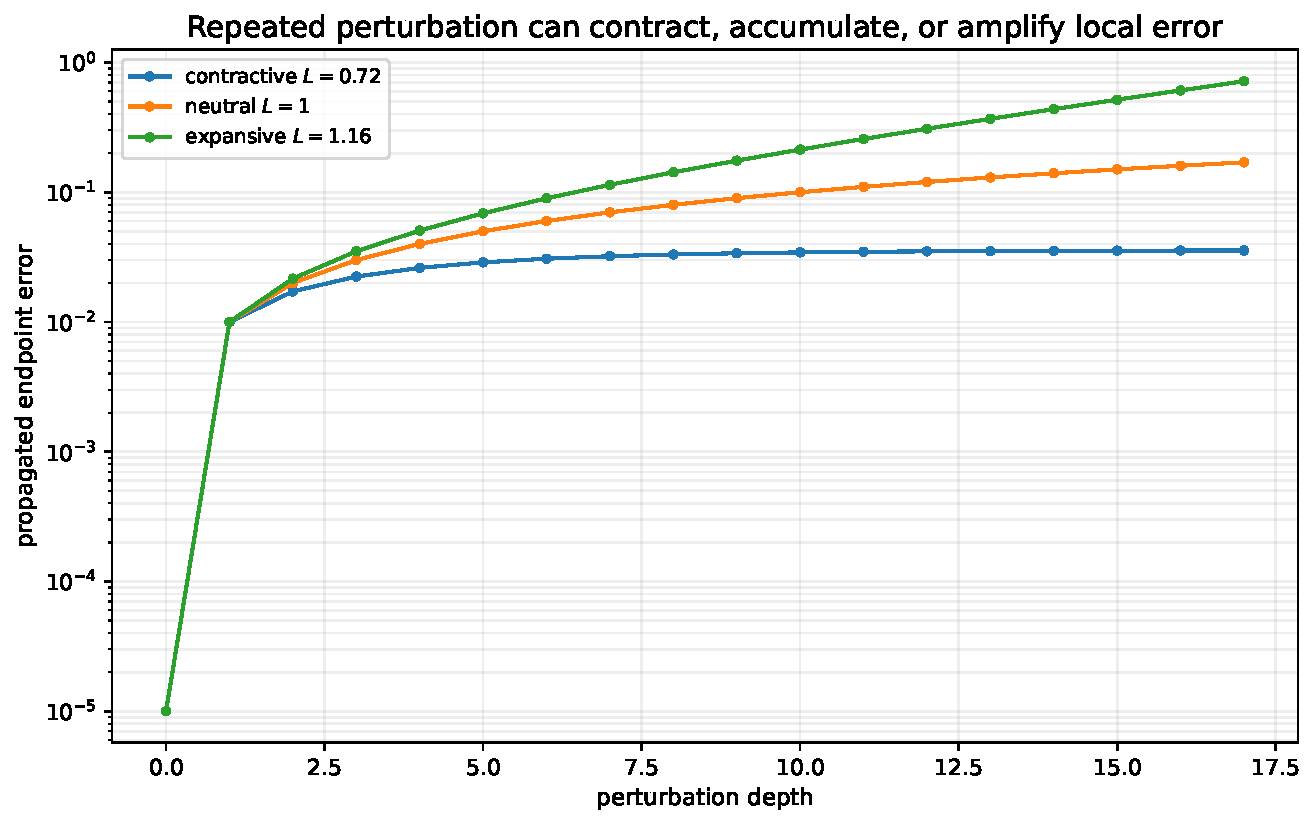
\includegraphics[width=0.98\textwidth]{18_stability_regimes.pdf}
\caption{The same local approximation error behaves differently under contractive, neutral, and expansive deformation laws. Stability is a property of the iterated sensitivities, not of depth alone.}
\label{fig:branch-stability}
\end{figure}

\section{Relation stability}

A quotient relation can change discontinuously under noise. Two exact eigenvalues may split. A zero symbolic identity may become a small residual. Therefore approximate quotienting must carry a margin or conditioning certificate.

\begin{boundary}[No threshold without a margin]
A numerical tolerance does not define a stable equivalence relation by itself. A reliable approximate quotient requires a separation gap, an interval certificate, exact arithmetic, or another proof that the classification is unchanged under the declared perturbation.
\end{boundary}

\chapter{Worked domain realizations}

The calculus is useful only when the abstract layers survive contact with concrete objects. The examples below use different state spaces, direction grammars, quotient relations, and completion rules. They are not presented as interchangeable models. Their common feature is the same audited production sequence:
\[
\text{seed}\longrightarrow\text{directions}\longrightarrow\text{raw routes}
\longrightarrow\text{quotient classes}\longrightarrow\text{certificate or completion}.
\]

\begin{longtable}{L{0.17\textwidth}L{0.29\textwidth}L{0.43\textwidth}}
\caption{Worked finite realizations in the visual-atlas edition.}\label{tab:worked-realizations}\\
\toprule
Domain & Seed and directions & What the quotient, certificate, or completion reveals \\
\midrule
\endfirsthead
\toprule
Domain & Seed and directions & What the quotient, certificate, or completion reveals \\
\midrule
\endhead
Integer walk & $0$ with $+1$ and $-1$ & $2^n$ routes collapse to $n+1$ endpoints, while exact binomial route multiplicities remain available. \\
Polynomials & $x^2+1$ with differentiation, translation, reflection, difference, and multiplication & Commuting and involutive operator routes become exact quotient relations between polynomial endpoints. \\
Analytic functions & $\cosh x$ with derivative, reciprocal, logarithmic derivative, parity, square, and doubling & Hyperbolic families, poles, singular descendants, and invalid operations coexist in one audited graph. \\
Sequences & A Fibonacci prefix and the impulse $\delta_0$ with difference, summation, binomial transform, sign alternation, and reversal & Exact transform relations generate structured integer families rather than one undifferentiated list of examples. \\
Gaussian laws & $N(0,1)$ with shift, scale, reflection, convolution, centering, and standardization & The relation-reduced atlas lives in exact $(\mu,\sigma^2)$ coordinates and exposes state-dependent canonicalization. \\
Matrices & $\left(\begin{smallmatrix}1&1\\0&1\end{smallmatrix}\right)$ with transpose, square, adjugate, conjugation, symmetrization, and commutator & Exact trace, determinant, rank, and symmetry metadata distinguish invariant-preserving routes from genuine deformation. \\
Affine shapes & A rational triangle with rotations, reflections, shear, scale, and translations & Concrete descendant geometry remains recursively deformable, with exact coordinate identities and finite-order symmetries. \\
Graphs & $P_3$ with complement, line graph, subdivision, leaf addition, and relabeling & Different labeled adjacency matrices collapse to canonical unlabeled graph-isomorphism classes. \\
Quantum states & The projective seed $|0\rangle$ with exact Bloch actions of $H,S,X,Z$ & Exponentially many gate words saturate at six Pauli eigenstates after global phase has been quotiented out. \\
Congruence lifts & Roots of $x^2=1$ over $3^m$ and $x^2=0$ over $2^m$ & Simple roots lift uniquely, while singular roots acquire state-dependent branching and dead ends. \\
Completion and products & Summable signed dyadic increments and multi-input products & Infinite routes receive limits only after completion, while Catalan syntax trees collapse only after associativity is imposed. \\
\bottomrule
\end{longtable}


\section{Polynomial operators and an exact commuting square}

Let
\[
p(x)=x^2+1,
\qquad
(Tp)(x)=p(x+1),
\qquad
(Dp)(x)=p'(x).
\]
The two primitive directions $T$ and $D$ satisfy
\[
D(Tp)=T(Dp)=2x+2.
\]
The raw path tree therefore contains two length-two routes,
\[
p\xrightarrow{T}Tp\xrightarrow{D}DTp,
\qquad
p\xrightarrow{D}Dp\xrightarrow{T}TDp,
\]
but the quotient graph contains one endpoint class because $DTp=TDp$ exactly.

\begin{figure}[H]
\centering
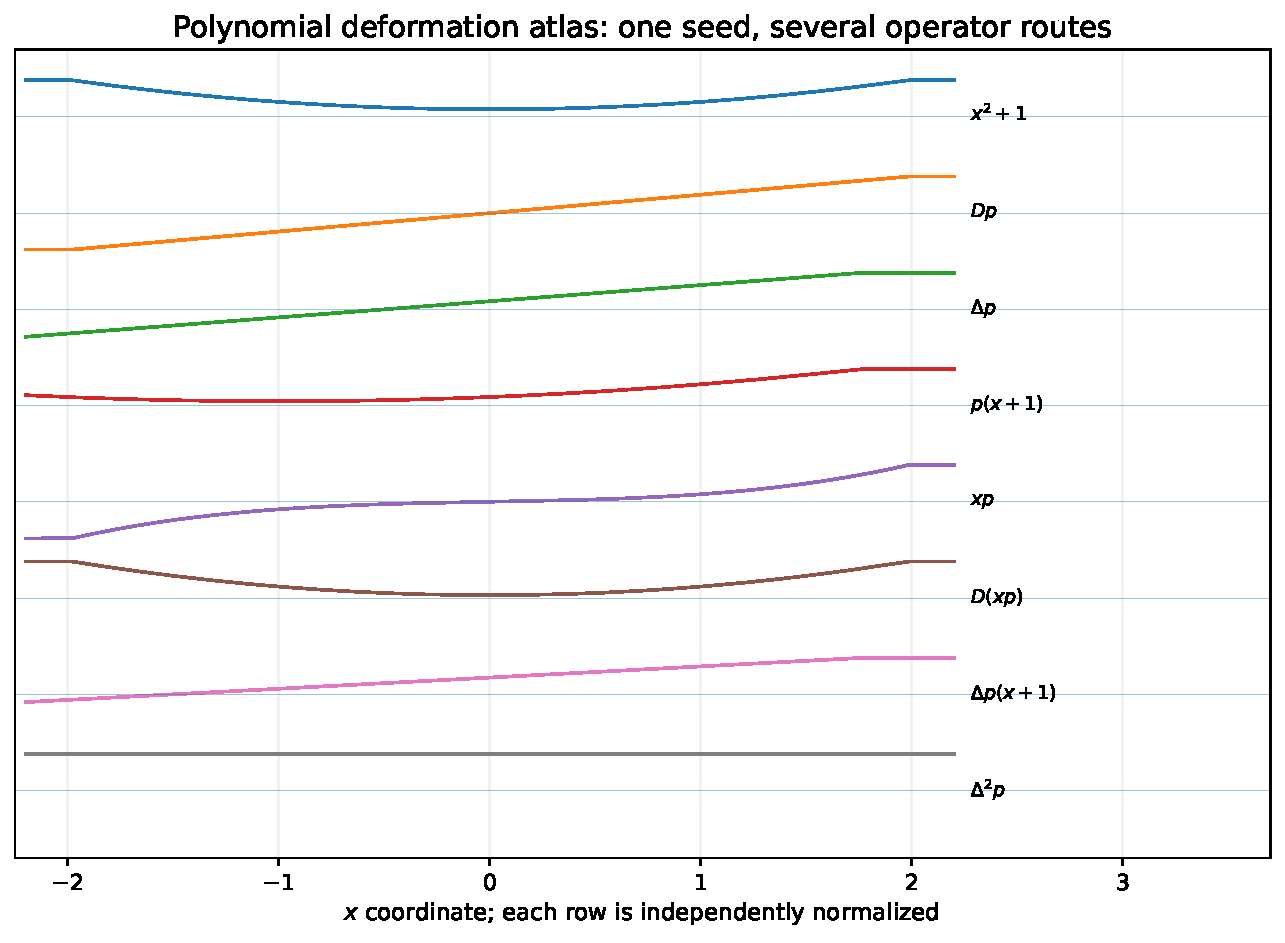
\includegraphics[width=0.98\textwidth]{09_polynomial_atlas.pdf}
\caption{Polynomial descendants are displayed as actual functions. Distinct operator routes are retained, while exact symbolic identities merge their endpoint classes.}
\label{fig:polynomial-square}
\end{figure}

The complete finite grammar used by the package also contains reflection, multiplication by $x$, and the forward finite difference. Starting from $x^2+1$, the depth-four experiment records \PolynomialRawPaths\ raw paths and \PolynomialQuotientNodes\ exact polynomial classes under coefficient canonicalization.

\section{Analytic functions from one hyperbolic seed}

Start from
\[
f_0(x)=\cosh x.
\]
The declared directions are differentiation, reciprocal formation, logarithmic differentiation, squaring, even projection, odd projection, and a restricted argument-doubling direction. The first three give
\[
D(\cosh x)=\sinh x,
\qquad
R(\cosh x)=\operatorname{sech}x,
\qquad
L(\cosh x)=\tanh x.
\]
Applying the same grammar again produces $\operatorname{csch}x$, $\coth x$, powers, parity components, and doubled arguments. Reciprocal and logarithmic derivative are rejected at the zero expression and the failed attempts remain in the audit.

\begin{figure}[H]
\centering
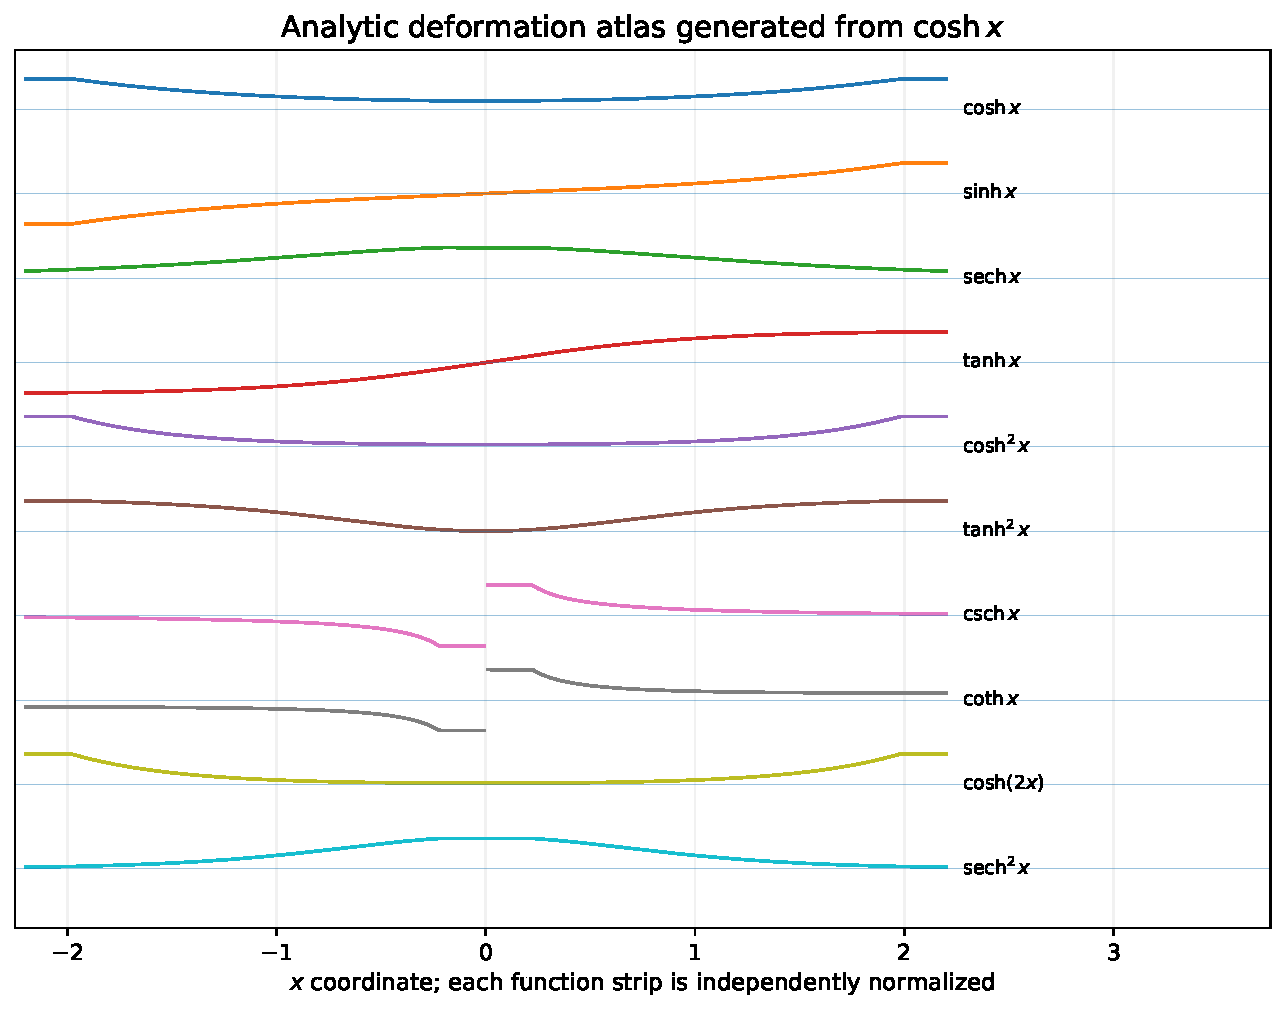
\includegraphics[width=0.99\textwidth]{10_analytic_atlas.pdf}
\caption{Analytic descendants are shown as a relation-reduced family of function profiles. Poles, parity projections, powers, derivatives, and logarithmic derivatives remain auditable.}
\label{fig:analytic-graph}
\end{figure}

\begin{table}[htbp]
\centering
\small
\caption{Selected analytic objects generated from the seed $\cosh x$.}
\label{tab:analytic-objects}
\begin{tabular}{rL{0.26\textwidth}L{0.48\textwidth}}
\toprule
Depth & Object & One shortest generating route \\
\midrule
0 & \texttt{\detokenize{cosh(x)}} & \texttt{\detokenize{seed}} \\
1 & \texttt{\detokenize{sinh(x)}} & \texttt{\detokenize{differentiate}} \\
1 & \texttt{\detokenize{1/cosh(x)}} & \texttt{\detokenize{reciprocal}} \\
1 & \texttt{\detokenize{tanh(x)}} & \texttt{\detokenize{log_derivative}} \\
1 & \texttt{\detokenize{cosh(2*x)}} & \texttt{\detokenize{double_argument}} \\
2 & \texttt{\detokenize{1/sinh(x)}} & \texttt{\detokenize{differentiate -> reciprocal}} \\
2 & \texttt{\detokenize{1/tanh(x)}} & \texttt{\detokenize{differentiate -> log_derivative}} \\
2 & \texttt{\detokenize{cosh(x)**(-2)}} & \texttt{\detokenize{reciprocal -> square}} \\
2 & \texttt{\detokenize{tanh(x)**2}} & \texttt{\detokenize{log_derivative -> square}} \\
2 & \texttt{\detokenize{tanh(2*x)}} & \texttt{\detokenize{log_derivative -> double_argument}} \\
\bottomrule
\end{tabular}
\end{table}


The recorded depth-three exploration contains \AnalyticRawPaths\ raw paths, \AnalyticQuotientNodes\ quotient objects, and twenty-four explicitly audited invalid attempts.

\section{Sequence transforms and a binomial subfamily}

The executable atlas starts from the eight-term Fibonacci prefix
\[
a=(0,1,1,2,3,5,8,13).
\]
Its fixed grammar contains first difference, partial summation, the binomial transform, sign alternation, and reversal. For a finite sequence $a=(a_0,\ldots,a_{N-1})$, define
\[
(Da)_0=a_0,
\qquad
(Da)_n=a_n-a_{n-1},
\]
\[
(Ca)_n=\sum_{j=0}^{n}a_j,
\qquad
(Ba)_n=\sum_{j=0}^{n}\binom{n}{j}a_j.
\]
The two triangular operators satisfy
\[
DC=CD=I
\]
on every finite sequence under the stated boundary convention. Hence the raw routes
\[
a\xrightarrow{D}Da\xrightarrow{C}CDa,
\qquad
a\xrightarrow{C}Ca\xrightarrow{D}DCa
\]
return to the seed class exactly.

A second, closed subfamily starts from the impulse $\delta=(1,0,0,\ldots)$. Repeated summation gives
\[
(C^k\delta)_n=\binom{n+k-1}{k-1}
\qquad(k\ge1),
\]
by induction and the hockey-stick identity. This provides a genuine family certificate: perturbation depth $k$ is the parameter, $C$ advances the parameter, $D$ reverses it away from the boundary, and the displayed coefficient formula is an exact invariant relation.

\begin{figure}[H]
\centering
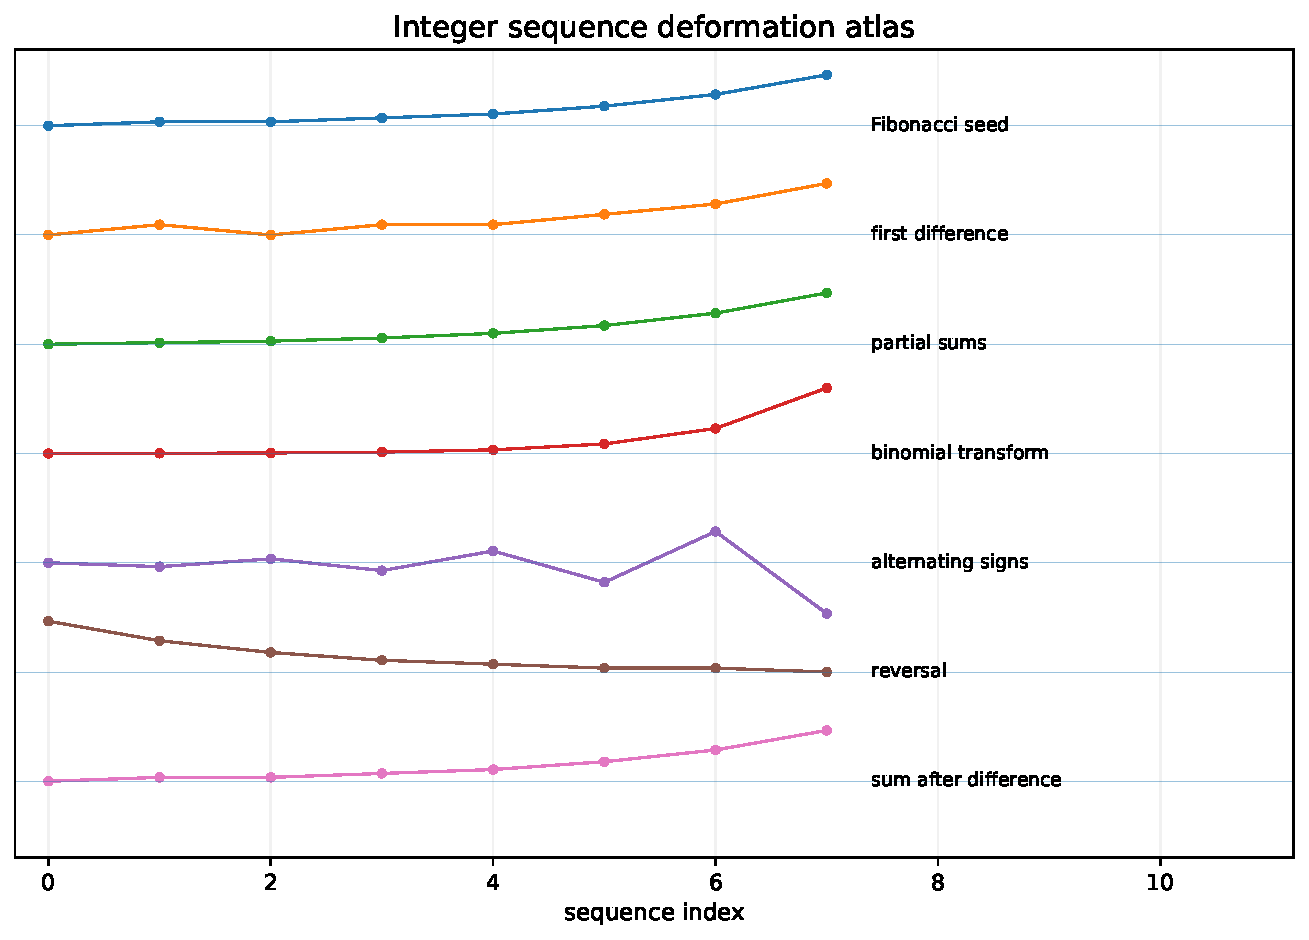
\includegraphics[width=0.99\textwidth]{11_sequence_atlas.pdf}
\caption{The finite Fibonacci seed is transformed by difference, summation, binomial weighting, sign alternation, and reversal. A separate impulse route yields the closed binomial subfamily $C^k\delta$.}
\label{fig:sequence-family}
\end{figure}

The depth-three finite exploration records \SequenceRawPaths\ raw paths, \SequenceQuotientNodes\ exact sequence states, and \SequenceQuotientEdges\ quotient edges. The visual uses the Fibonacci seed because it exposes all five transforms in one compact finite example. The binomial formula supplies the accompanying infinite parameterized example.

\section{Gaussian probability laws}

Represent a one-dimensional Gaussian law by the exact parameter pair $(\mu,v)$, where $v=\sigma^2>0$. The grammar contains shifts by $\pm1$, reflection, convolution with $N(0,1)$, centering, scaling by two, and standardization. Their parameter actions are
\[
\begin{aligned}
(\mu,v)&\mapsto(\mu\pm1,v),
& (\mu,v)&\mapsto(-\mu,v),\\
(\mu,v)&\mapsto(\mu,v+1),
& (\mu,v)&\mapsto(0,v),\\
(\mu,v)&\mapsto(2\mu,4v),
& (\mu,v)&\mapsto(0,1).
\end{aligned}
\]
Standardization is state dependent: it is exposed only away from the canonical seed. Reflection is invisible at centered laws, while convolution and scaling change entropy through the variance coordinate.

One explicit route is
\[
(0,1)\xrightarrow{\text{shift }+1}(1,1)
\xrightarrow{\ast N(0,1)}(1,2)
\xrightarrow{\text{scale }2}(2,8)
\xrightarrow{\text{standardize}}(0,1).
\]
The final edge is a many-to-one canonicalization direction. It produces a strong quotient collapse without erasing the route that created the noncanonical law. The differential entropy
\[
h(N(\mu,v))=\frac12\log(2\pi e v)
\]
is unaffected by shifts and reflection, increases under unit convolution, and changes by $\log 2$ under scaling by two.

\begin{figure}[H]
\centering
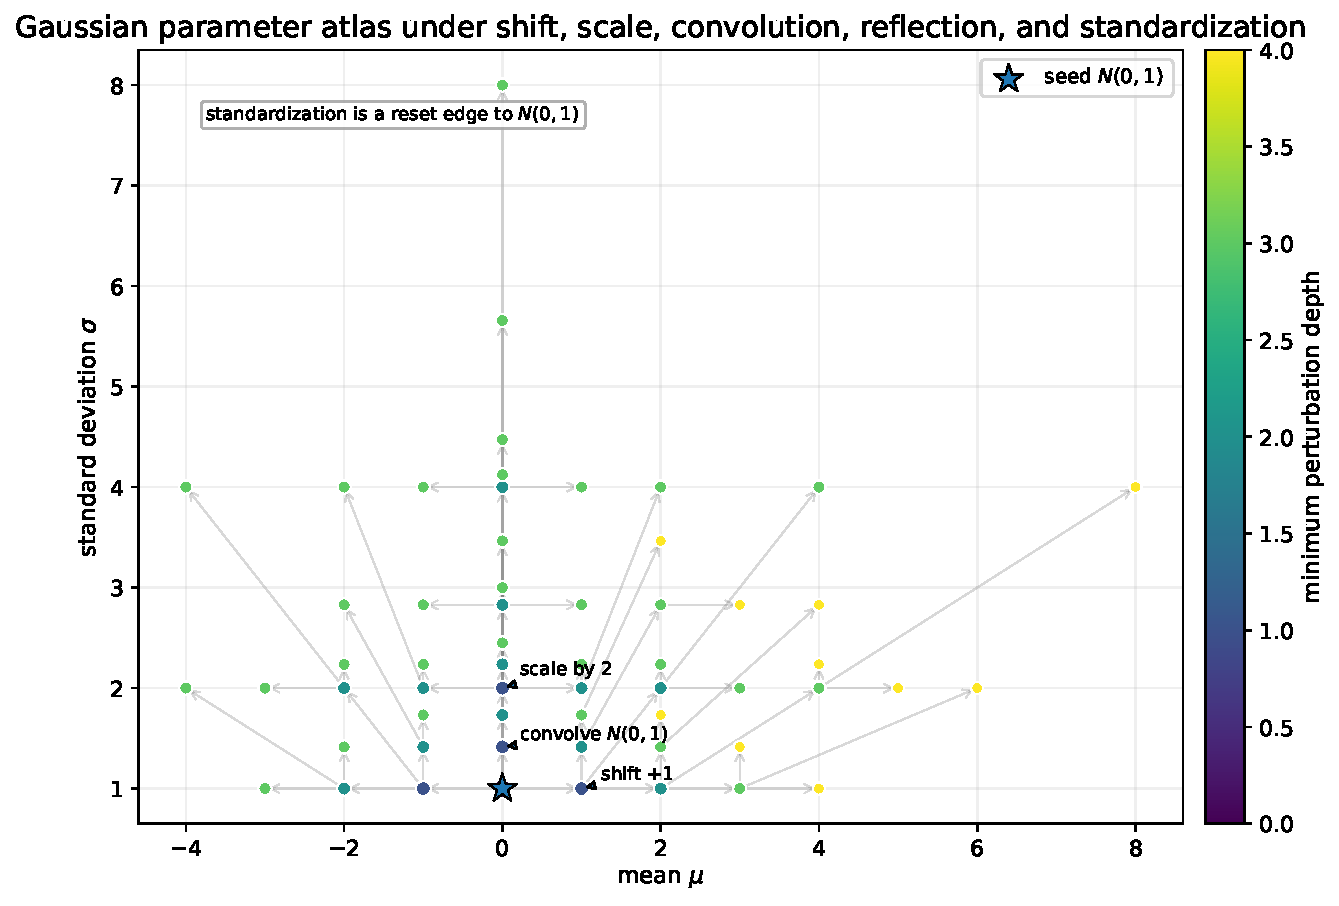
\includegraphics[width=0.99\textwidth]{12_gaussian_atlas.pdf}
\caption{The Gaussian atlas is plotted in mean and standard-deviation coordinates. Color records minimum perturbation depth. A shortest-route forest retains construction history without obscuring the exact parameter geometry.}
\label{fig:gaussian-atlas}
\end{figure}

The recorded prefix contains \GaussianRawPaths\ raw paths, \GaussianQuotientNodes\ exact parameter pairs, and \GaussianQuotientEdges\ quotient edges.

\section{Graph deformation modulo isomorphism}

Begin with the path graph $P_3$ on three vertices. The finite grammar contains graph complement, line-graph formation, leaf attachment, edge subdivision, and a relabeling direction. Raw states are labeled adjacency matrices. For a graph with $n\le6$ vertices, the quotient key is the lexicographically least adjacency bit string over all $n!$ vertex permutations.

This example distinguishes two kinds of movement. Complement and line-graph formation can create genuinely new graph classes. A relabeling changes the raw adjacency matrix but not the quotient object. Subdivision and leaf attachment also change the number of vertices, so the direction fiber depends on the current graph rather than only on the original seed.

For the seed $P_3$, the first descendants include
\[
\overline{P_3},
\qquad
L(P_3)\cong P_2,
\qquad
P_3\text{ with one attached leaf},
\qquad
P_4\text{ obtained by subdivision}.
\]
If $\rho$ reverses the vertex labels, then
\[
\operatorname{key}(G)=\operatorname{key}(\rho G\rho^{-1})
\]
exactly, although the two raw paths and raw adjacency matrices remain distinct.

\begin{figure}[H]
\centering
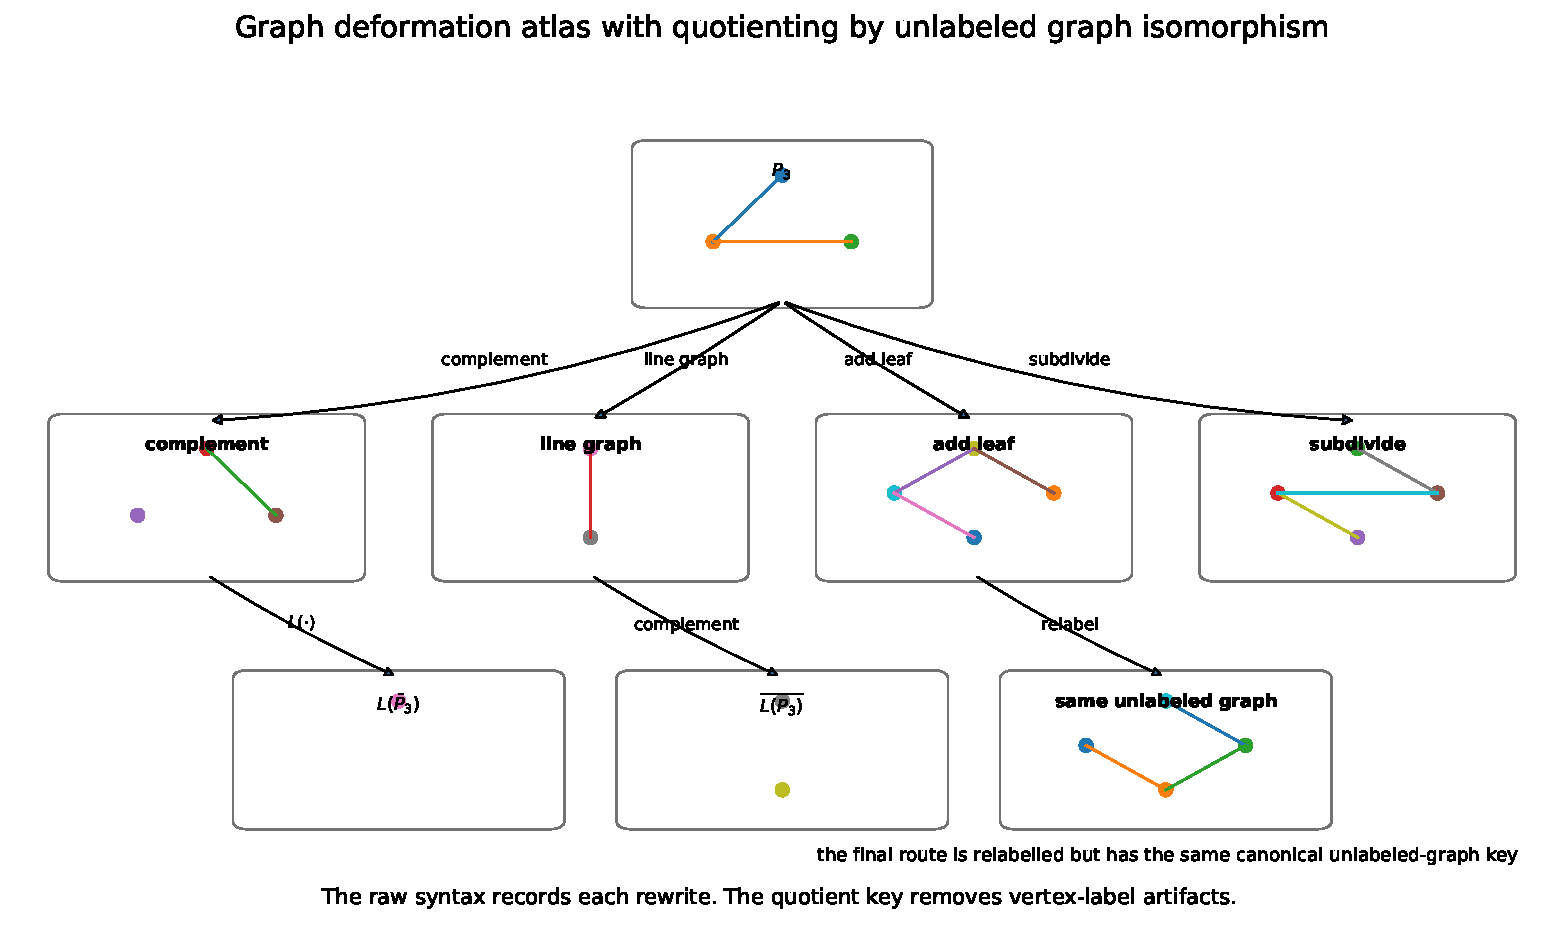
\includegraphics[width=0.99\textwidth]{16_graph_atlas.pdf}
\caption{Graph directions include complement, line graph, subdivision, leaf addition, and relabeling. Separated cards keep each graph legible, while exact canonicalization merges labeled routes representing the same unlabeled graph.}
\label{fig:graph-quotient}
\end{figure}

The recorded prefix contains \GraphRawPaths\ raw paths, \GraphQuotientNodes\ quotient graph classes, and \GraphQuotientEdges\ directed quotient edges.

\section{Finite matrix deformation atlas}

Let
\[
A_0=\begin{pmatrix}1&1\\0&1\end{pmatrix}.
\]
The declared matrix directions are transpose, negation, squaring, conjugation by the coordinate swap, symmetrization, commutation with
\[
J=\begin{pmatrix}0&-1\\1&0\end{pmatrix},
\]
and adjugation. Every result is stored as an exact integer matrix. The metadata include trace, determinant, rank, symmetry, and squared Frobenius norm.

The first calculations are explicit:
\[
A_0^{\mathsf T}=\begin{pmatrix}1&0\\1&1\end{pmatrix},
\qquad
A_0^2=\begin{pmatrix}1&2\\0&1\end{pmatrix},
\qquad
\operatorname{adj}(A_0)=\begin{pmatrix}1&-1\\0&1\end{pmatrix}.
\]
They satisfy
\[
(A^{\mathsf T})^{\mathsf T}=A,
\qquad
A\operatorname{adj}(A)=\det(A)I,
\qquad
\det(SAS)=\det(A)
\]
for the swap matrix $S$. Thus involution, adjugate, and conjugacy relations generate quotient identifications, while squaring and commutation usually move to new invariant values.

\begin{figure}[H]
\centering
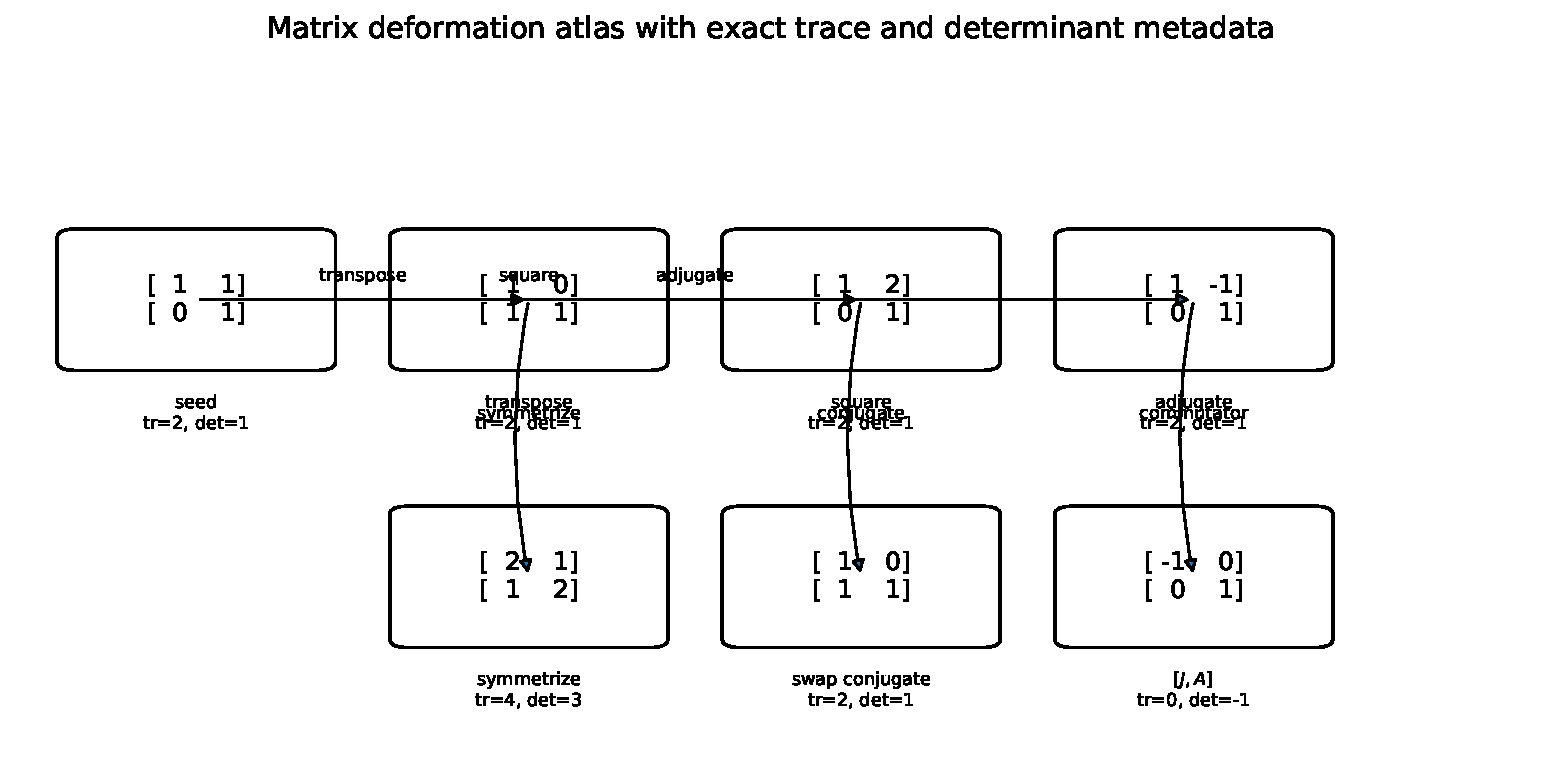
\includegraphics[width=0.99\textwidth]{15_matrix_atlas.pdf}
\caption{Each matrix descendant is displayed with exact trace and determinant. Transposition, squaring, adjugation, symmetrization, conjugation, and commutation create an audited operator atlas.}
\label{fig:matrix-quotient}
\end{figure}

The recorded prefix contains \MatrixRawPaths\ raw paths, \MatrixQuotientNodes\ exact matrix objects, and \MatrixQuotientEdges\ quotient edges.

\section{A single-qubit gate orbit}

The implementation works directly after quotienting global phase. A state is one of the six exact Bloch-axis vectors
\[
(0,0,\pm1),
\qquad
(\pm1,0,0),
\qquad
(0,\pm1,0),
\]
representing the Pauli eigenstates $|0\rangle$, $|1\rangle$, $|+\rangle$, $|-\rangle$, $|+i\rangle$, and $|-i\rangle$. The primitive grammar contains $H,S,X,Z$, acting as signed permutations of the Bloch coordinates:
\[
H(x,y,z)=(z,-y,x),
\qquad
S(x,y,z)=(-y,x,z),
\]
\[
X(x,y,z)=(x,-y,-z),
\qquad
Z(x,y,z)=(-x,-y,z).
\]
These rules are exact and avoid floating-point phase canonicalization.

Starting from $|0\rangle$, one has
\[
|0\rangle\xrightarrow{H}|+\rangle
\xrightarrow{S}|+i\rangle
\xrightarrow{S}|-\rangle,
\]
while $H^2=X^2=Z^2=I$ on the projective orbit and $S^4=I$. The number of raw gate words grows as $4^n$, but the quotient orbit saturates at six objects.

\begin{figure}[H]
\centering
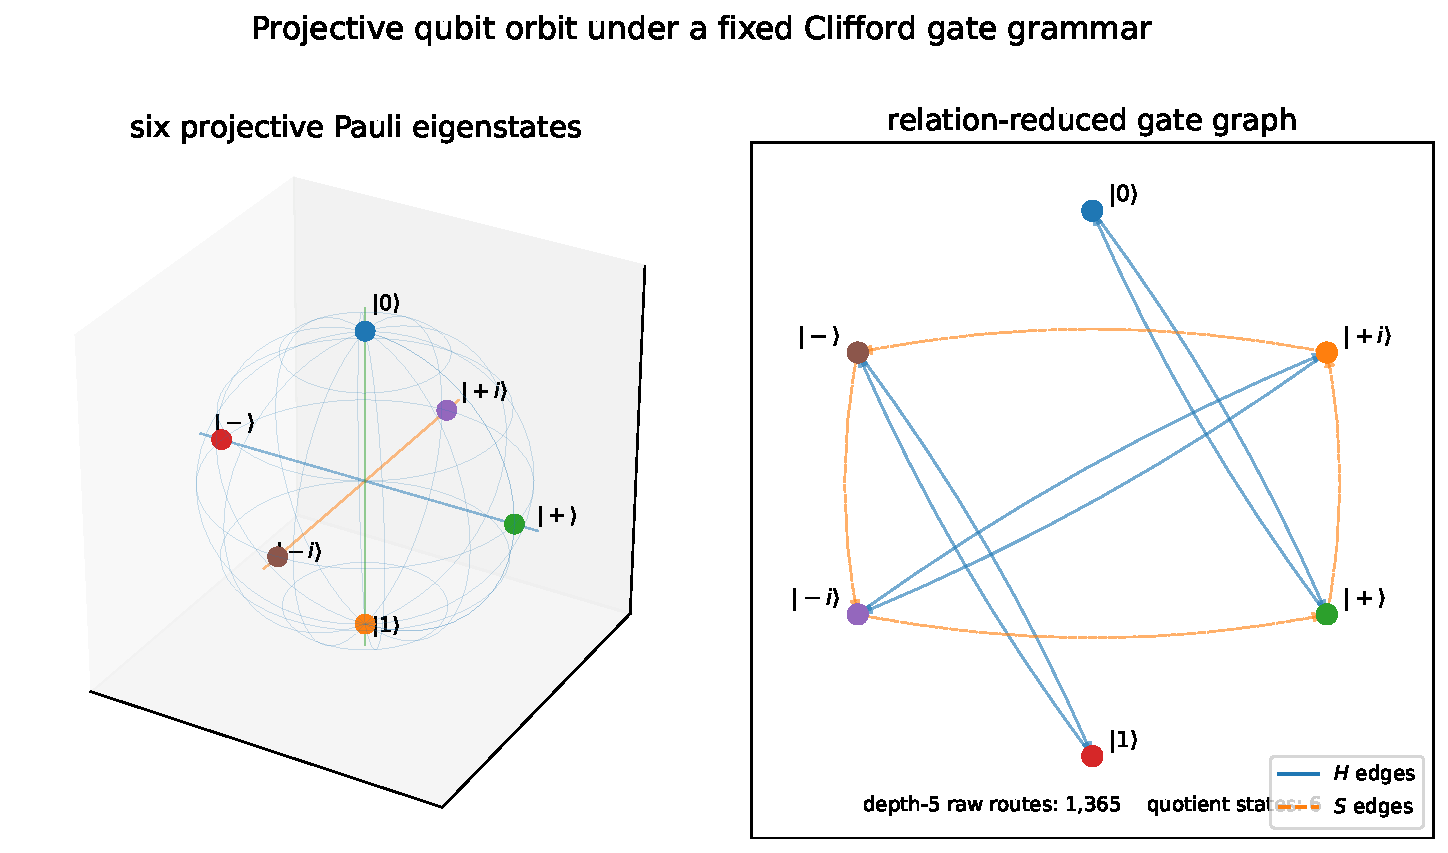
\includegraphics[width=0.99\textwidth]{13_qubit_atlas.pdf}
\caption{The left panel realizes the quotient states on the Bloch sphere. The right panel shows the relation-reduced gate graph for the displayed $H$ and $S$ generators.}
\label{fig:qubit-orbit}
\end{figure}

The depth-five prefix contains \QubitRawPaths\ raw gate words, \QubitQuotientNodes\ quotient states, and \QubitQuotientEdges\ quotient edges.

\section{Affine geometry with descendant-specific directions}

Take the rational triangle
\[
K_0=\left\{(0,0),(2,0),\left(1,\frac32\right)\right\}.
\]
The grammar contains quarter turns, reflection in the $x$ axis, horizontal shear, scaling by two, and unit translations in the two coordinate directions. Each descendant is again a finite rational point configuration, so the grammar is queried recursively at every child.

For example,
\[
R(x,y)=(-y,x),
\qquad
H(x,y)=(x+y,y),
\qquad
S_2(x,y)=(2x,2y).
\]
The relation $R^4=I$ closes one route loop exactly. Reflection is an involution. Rotation preserves signed area, reflection reverses its sign, shear preserves it, and scaling by two multiplies it by four. These invariants separate visually similar but mathematically different descendants.

\begin{figure}[H]
\centering
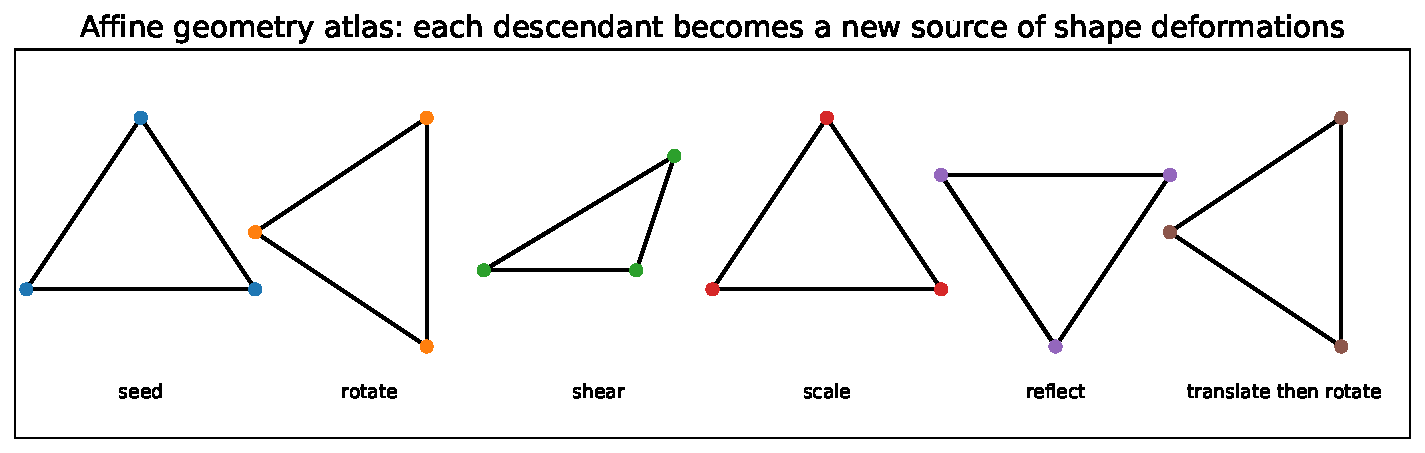
\includegraphics[width=0.99\textwidth]{14_affine_shape_atlas.pdf}
\caption{Affine descendants are plotted as concrete shapes. Every child remains a parent for further rotations, reflections, shears, scales, and translations.}
\label{fig:shape-atlas}
\end{figure}

The explored prefix contains \ShapeRawPaths\ raw paths, \ShapeQuotientNodes\ exact shape states, and \ShapeQuotientEdges\ quotient edges.

\section{Completion of a summable perturbation branch}

The executable completion example starts from $x_0=0$ and exposes the two depth-dependent directions
\[
d_n^{\pm}=\pm2^{-(n+1)}.
\]
A finite route with signs $\varepsilon_n\in\{-1,+1\}$ reaches
\[
x_N=\sum_{n=0}^{N-1}\varepsilon_n2^{-(n+1)}.
\]
Every infinite sign route is Cauchy because
\[
|x_m-x_n|
\le
\sum_{k=n}^{m-1}2^{-(k+1)}
<2^{-n}.
\]
The completed object therefore contains a limit for every infinite route. The selected periodic sign pattern used in the figure converges numerically to $5/7$.

The numerical convergence and the certified tail envelope are displayed in \cref{fig:branch-convergence}.

The same architecture covers iterated function systems. For the middle-third Cantor maps $L(x)=x/3$ and $R(x)=(x+2)/3$, finite words identify cylinder intervals and infinite words receive points only in the completed boundary. The dyadic example is used in the executable release because its exact tail certificate is especially transparent.

\section{Associative multi-input products}

With four ordered leaves and one binary operation, the free operadic layer contains the five Catalan parenthesizations
\[
((ab)c)d,
\quad
(a(bc))d,
\quad
(ab)(cd),
\quad
a((bc)d),
\quad
a(b(cd)).
\]
They are different syntax trees. If the operation is associative, all five evaluate to one quotient object. If it is also commutative, the $4!$ permutations of the leaves are identified as well. The raw tree and the quotient must therefore remain separate even in elementary algebra. The complete syntax-to-quotient visual appears in \cref{fig:operadic}.

\section{Congruence lifting and singular branch geometry}

For a prime $p$, a state at level $m$ is a residue class modulo $p^m$ satisfying a declared congruence. Its direction fiber is the finite set of next base-$p$ digits that lift the current solution to level $m+1$.

For $x^2=1$ over powers of $3$, the two simple roots lift uniquely:
\[
1\pmod 3\longleftarrow1\pmod 9\longleftarrow1\pmod{27}\longleftarrow\cdots,
\]
\[
-1\pmod 3\longleftarrow-1\pmod 9\longleftarrow-1\pmod{27}\longleftarrow\cdots.
\]
For the singular equation $x^2=0$ over powers of $2$, some nodes have several valid next digits and some branches later die. Thus branching number is an object property detected by the local congruence geometry.

\begin{figure}[H]
\centering
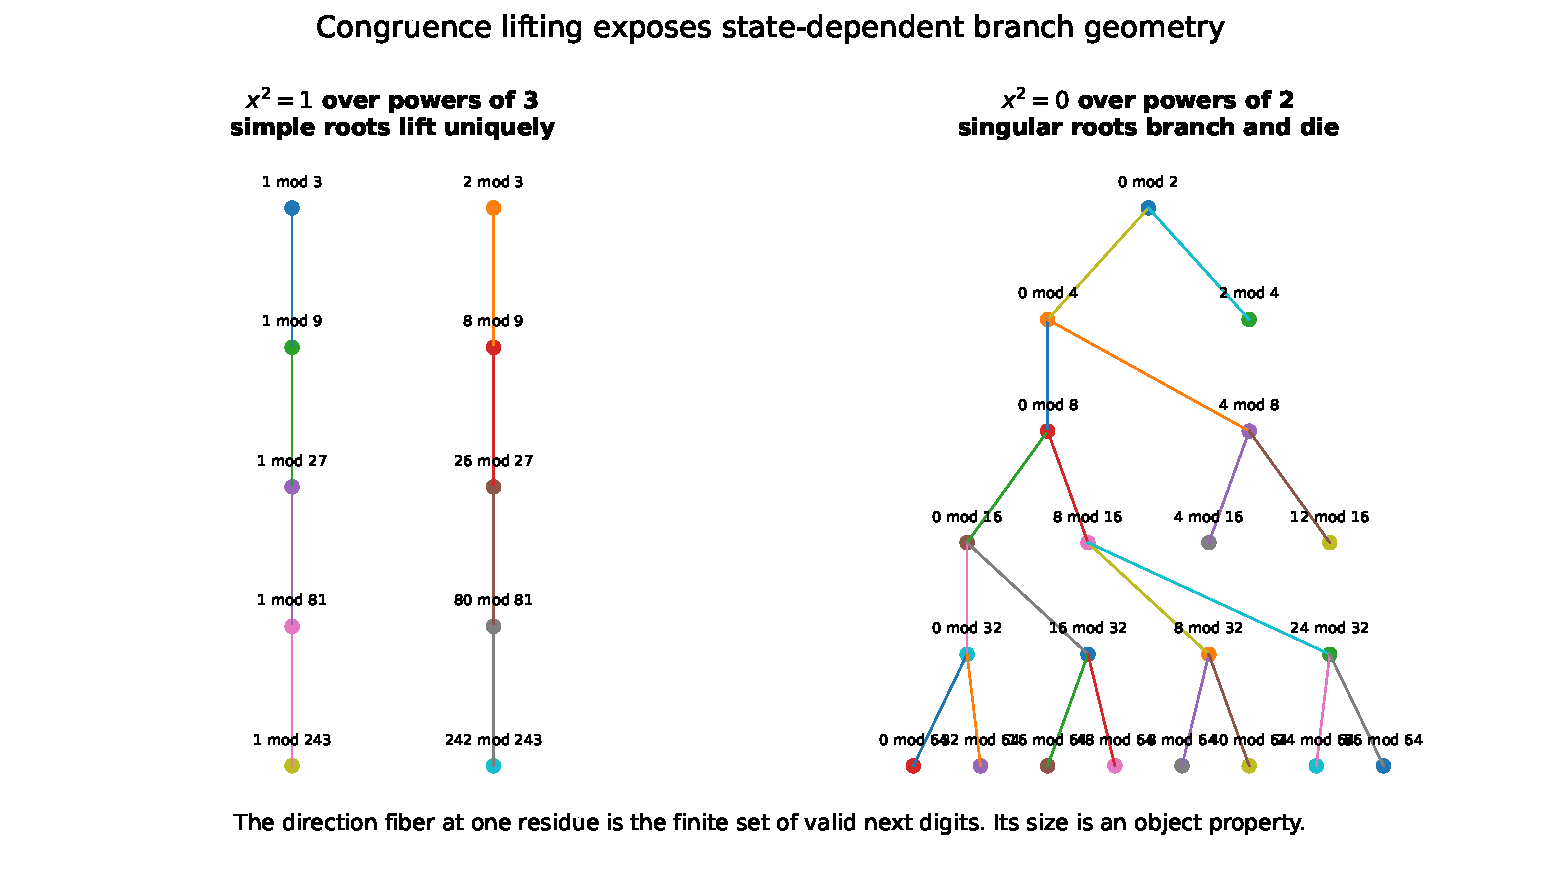
\includegraphics[width=0.99\textwidth]{17_adic_lift_forest.pdf}
\caption{Simple roots produce unique lift streams, whereas singular roots branch and terminate. The direction fiber at each node is the exact set of valid next digits.}
\label{fig:adic-lifts}
\end{figure}

The two recorded prefixes contain \AdicSimpleRawPaths\ simple-lift routes and \AdicSingularRawPaths\ singular-lift routes.

\section{Cross-domain route compression}

The eleven realizations use different grammars and quotient relations. Their raw-path counts and quotient-object counts should therefore not be compared as one performance benchmark. The comparison is structural: it shows how strongly relations can compress the same finite-depth exploration.

\begin{figure}[H]
\centering
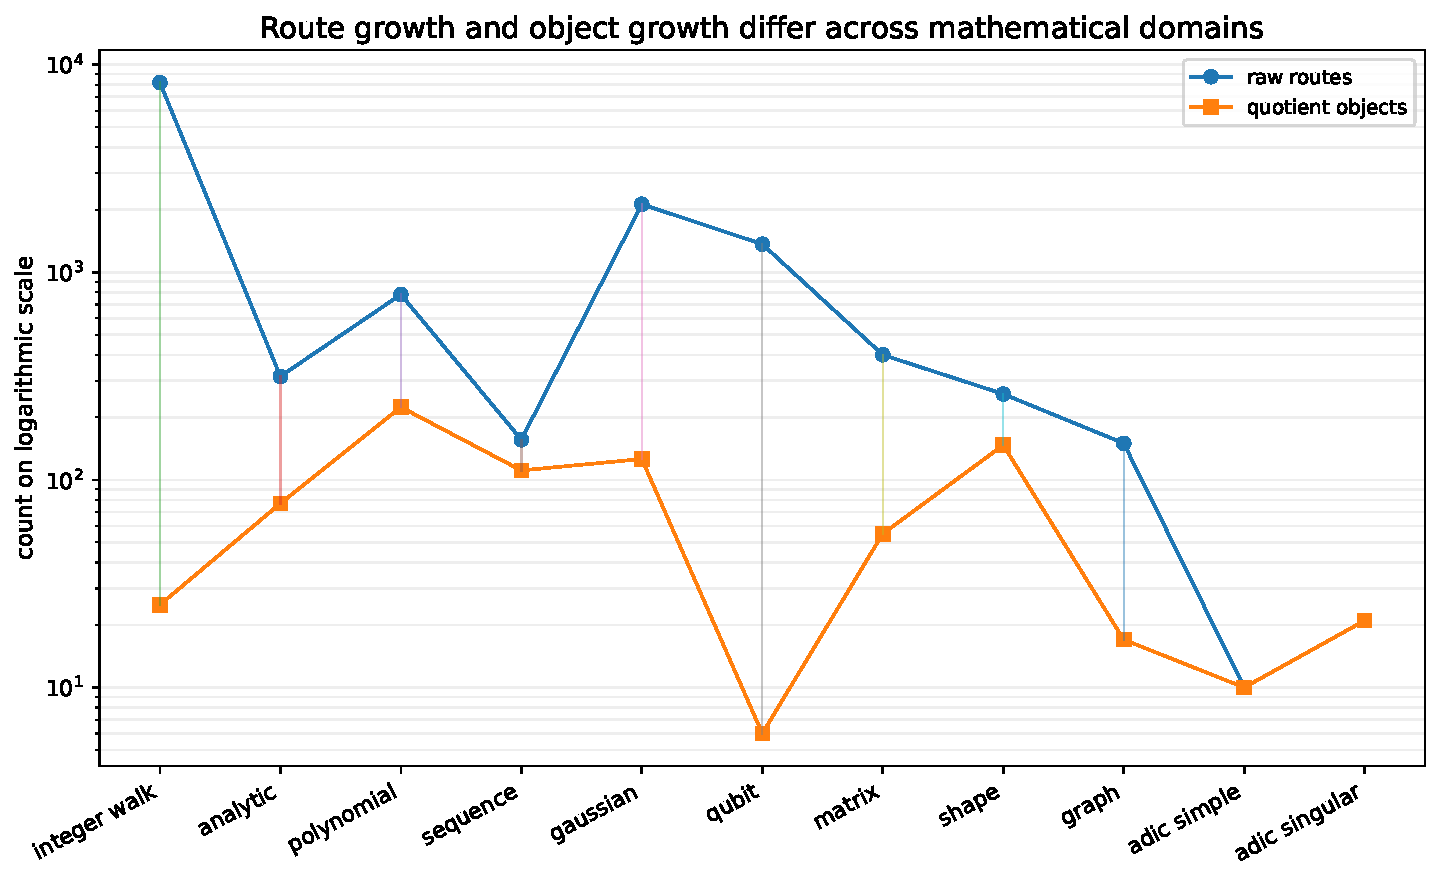
\includegraphics[width=0.99\textwidth]{19_cross_domain_counts.pdf}
\caption{Raw route growth and quotient-object growth can differ by orders of magnitude. Strong collapse occurs for the integer walk and projective qubit orbit, while the finite sequence and shape grammars retain more distinct descendants.}
\label{fig:cross-domain-counts}
\end{figure}

\begin{longtable}{lrrrr}
\caption{Finite explored prefixes used in the visual atlas.}\label{tab:example-summary}\\
\toprule
Example & Raw paths & Quotient nodes & Edges & Invalid \\
\midrule
\endfirsthead
\toprule
Example & Raw paths & Quotient nodes & Edges & Invalid \\
\midrule
\endhead
integer walk & 8191 & 25 & 46 & 0 \\
analytic & 315 & 77 & 149 & 24 \\
polynomial & 781 & 224 & 355 & 0 \\
sequence & 156 & 111 & 135 & 0 \\
gaussian & 2125 & 126 & 335 & 0 \\
qubit & 1365 & 6 & 24 & 0 \\
matrix & 400 & 55 & 161 & 0 \\
shape & 259 & 147 & 210 & 0 \\
graph & 150 & 17 & 41 & 0 \\
$p$-adic simple & 10 & 10 & 8 & 0 \\
$p$-adic singular & 21 & 21 & 20 & 0 \\
\bottomrule
\end{longtable}


\section{What the examples establish}

These examples cover several distinct reasons for quotienting, certification, and completion:
\begin{itemize}
\item equal endpoints reached by different paths
\item operator commutation
\item symbolic analytic identities
\item inverse transformation laws
\item graph isomorphism
\item conjugacy invariance
\item global quantum phase
\item associativity of multi-input operations
\end{itemize}
They also show two distinct uses of completion: summable perturbation streams and iterated contraction systems. None of the examples proves that a useful quotient or completion exists in every domain. Each one demonstrates how the required domain theorem enters the common calculus.

\chapter{Implementation and verification}

\section{Package architecture}

The package \texttt{komorebi-generative-deformation} is organized around a small interface.

\begin{longtable}{L{0.28\textwidth}L{0.62\textwidth}}
\caption{Core software objects.}\label{tab:api}\\
\toprule
Object & Role \\
\midrule
\endfirsthead
\toprule
Object & Role \\
\midrule
\endhead
\texttt{DeformationSystem} & Supplies state-dependent directions, one-step application, canonical keys, invariants, validation, serialization, and optional distance.\\
\texttt{Direction} & Stores a primitive direction label, parameter, cost, family name, resolution, and metadata.\\
\texttt{PerturbationForest} & Stores raw paths, relation-reduced nodes, directed edges, multiplicities, invalid attempts, and export methods.\\
\texttt{ExplorationConfig} & Declares depth, path, node, edge, strategy, and per-path direction limits.\\
\texttt{IntervalDirectionFamily} & Represents a continuous interval of directions through dyadic certified nets.\\
\texttt{InteractionRule} & Declares a multi-input deformation for the operadic hyperforest.\\
\texttt{FamilyCertificate} & Stores parameter assignments, closure directions, relations, invariants, and verification failures.\\
\texttt{metrics} & Implements entropy proxies, growth series, partition functions, cover error, and tail bounds.\\
\bottomrule
\end{longtable}

\section{Reference experiments}

The complete experiment driver rebuilds every forest, every table, and all \FigureCount\ vector-PDF and PNG figure pairs from source. The eleven relation-reduced finite prefixes are summarized in \cref{tab:example-summary}. They should not be read as a speed ranking because their grammars, depth limits, state spaces, and quotient relations are different.

The \BuiltInChecks\ built-in checks verify:
\begin{itemize}
\item exact raw and quotient growth for the integer walk
\item the dyadic completion tail bound
\item monotone decay of the continuous-direction cover error
\item Catalan and Fibonacci identities
\item generation of $\tanh x$ and $\operatorname{sech}x$
\item inverse sequence transforms
\item Gaussian standardization
\item six-state projective qubit closure
\item purity preservation
\item matrix and affine involutions
\item graph relabeling invariance
\item unique simple-root lifting and singular-root branching
\end{itemize}
All \BuiltInChecks\ checks pass in the recorded run. The result file stores every Boolean check separately rather than recording only a final aggregate.

\section{Independent test suite}

The independent suite contains \TestCount\ tests. The tests are grouped by mathematical contract rather than by figure:

\begin{longtable}{L{0.25\textwidth}L{0.64\textwidth}}
\caption{Independent verification groups.}\label{tab:test-groups}\\
\toprule
Group & Representative assertions \\
\midrule
\endfirsthead
\toprule
Group & Representative assertions \\
\midrule
\endhead
Forest accounting & Raw binary path counts, quotient counts, route multiplicity, shortest paths, invalid-attempt audit, and export round trips.\\
Completion and covers & Dyadic Cauchy behavior, interval-net coverage, geometric tail estimates, and propagated finite-cover error.\\
Family certificates & Catalan and Fibonacci values, exact recurrence inference, rejection of false recurrences, invariant clustering, and closure checks.\\
Multi-input structure & Binary addition and multiplication, ternary interaction limits, and preservation of syntax-tree distinctions before quotienting.\\
Symbolic examples & Polynomial route collapse, analytic generation of $\tanh$ and $\operatorname{sech}$, and explicit rejection of invalid reciprocal operations.\\
Extended domains & Sequence inverses, Gaussian parameter actions, six-state qubit closure and purity, matrix adjugation and involutions, affine symmetry, graph isomorphism, and simple versus singular congruence lifting.\\
\bottomrule
\end{longtable}

The recorded run passes all \TestCount\ tests. The tests do not infer unbounded correctness from finite execution. They verify the exact finite contracts exported by the release and support the manuscript's concrete examples.

\section{Machine-readable audit trail}

Every explored example exports:

\begin{itemize}
\item \texttt{forest.json} with nodes, edges, summaries, paths, and failures
\item \texttt{nodes.csv} with states, invariants, costs, and shortest routes
\item \texttt{edges.csv} with directions, depth, cost, and multiplicity
\item generated figures in vector PDF and PNG formats
\item exact test and experiment summaries
\end{itemize}

The invalid-attempt log is part of the mathematical record. A missing reciprocal, failed constraint, or complexity cap is not treated as an absent direction without explanation.

\chapter{What the calculus does and does not claim}

\section{What has been completed}

Version 1.1.0 contains \FigureCount\ Python-generated figure pairs and \ExampleCount\ worked domain realizations. The final generative object consists of the following linked structures.

\begin{enumerate}[label=(\arabic*)]
\item A typed object space with one direction fiber at every object.
\item A raw rooted forest containing every finite admissible route.
\item A relation quotient that separates path multiplicity from distinct object classes.
\item A completion rule for infinite compatible routes.
\item A parameter-cover theorem for continuous direction families.
\item An operadic extension for multi-input interactions.
\item Exact path projectors and refinement identities.
\item Growth entropy and weighted path partition functions.
\item A family certificate with closure, relations, and invariants.
\item A finite explorer that preserves paths, quotient nodes, failures, and residual uncertainty.
\end{enumerate}

\section{What remains domain dependent}

The abstract calculus cannot decide which directions are mathematically natural in every subject. It cannot supply a topology when a domain has not chosen one. It cannot infer an exact quotient from an unstable numerical similarity. It cannot guarantee that a family is historically new. It cannot make an infinite uncountable fiber finite.

These are not defects in the definition. They are the information that a valid realization must provide.

\section{Meaning of universal}

Universal means that the same construction accepts many typed realizations. It does not mean that one fixed finite direction list reaches every mathematical object. A universal interface can still require different domain grammars.

\begin{boundary}[No metaphysical enumeration]
There is no literal operation that tries every conceivable direction in all of mathematics. The formal replacement is exact: declare the admissible direction object, prove that the grammar contains the directions relevant to the domain, and explore finite or parameterized prefixes with coverage certificates.
\end{boundary}

\begin{boundary}[No finite proof of an infinite search claim]
A finite run proves only the statements certified for that run. Infinite completeness comes from theorems about the grammar, fairness, compactness, convergence, and relations. It does not follow from a large node count.
\end{boundary}

\begin{boundary}[No novelty from generation alone]
Generating an expression along an unfamiliar route does not make the expression new. A novelty claim requires comparison with known objects, transformations, parameterizations, and identities.
\end{boundary}

\chapter{Conclusion}

The proposed object can be summarized in one line:
\[
\boxed{
\begin{gathered}
\text{object}
\longrightarrow
\text{all declared directions at that object}
\longrightarrow
\text{all directions at every child}
\\[0.25em]
\longrightarrow
\text{path forest}
\longrightarrow
\text{relation quotient}
\longrightarrow
\text{completed family universe}.
\end{gathered}
}
\]

The phrase perturbations of perturbations is therefore not shorthand for a second derivative. It is a recursive closure rule whose local direction space changes with the object. Finite words describe unary routes. Rooted operation trees describe nonlinear interactions. Relations identify different constructions of the same object. Completion gives meaning to infinite routes. Projectors retain local route information. Family certificates identify parameterized structures inside the generated universe.

This is the final generative framework implemented in the accompanying release. It is broad enough to express algebraic, analytic, geometric, signal, stochastic, quantum, and arithmetic deformation systems, while remaining strict about admissibility, equivalence, convergence, and auditability.

\appendix

\chapter{Compact formula registry}

\begin{longtable}{L{0.31\textwidth}L{0.58\textwidth}}
\caption{Core formula registry.}\label{tab:formula-registry}\\
\toprule
Object & Definition or identity \\
\midrule
\endfirsthead
\toprule
Object & Definition or identity \\
\midrule
\endhead
Direction fiber & $\Dcal_x=\pi^{-1}(x)$ \\
One-step deformation & $x\star d=\Phi(d)$ for $d\in\Dcal_x$ \\
Length-$n$ path layer & $\Tcal_n(x_0)$ \\
Endpoint map & $\ev(d_1,\ldots,d_n)=x_n$ \\
Raw finite forest & $\Tcal_{\mathrm{fin}}(x_0)=\coprod_{n\ge0}\Tcal_n(x_0)$ \\
Path cost & $\cost(\gamma)=\sum_k\kappa(d_k)$ \\
Quotient object graph & $\Ocal(x_0)=\Tcal_{\mathrm{fin}}(x_0)/\sim$ \\
Infinite boundary & $\partial\Tcal(x_0)$ \\
Cover recursion & $e_k\le L_ke_{k-1}+M_k\epsilon_k$ \\
Cover closed bound & $e_n\le (\prod L_k)e_0+\sum_jM_j\epsilon_j\prod_{k>j}L_k$ \\
Summable branch condition & $d(x_{n+1},x_n)\le a_n$, $\sum a_n<\infty$ \\
Cylinder projector & $P^{(n)}_\alpha\lvert\gamma\rangle=1_{\alpha\preceq\gamma}\lvert\gamma\rangle$ \\
Projector refinement & $P_\alpha=\sum_dP_{\alpha d}$ \\
Transfer block & $A_{\beta\alpha}=Q_\beta A P_\alpha$ \\
Path product law & $(BA)_{\gamma\alpha}=\sum_\beta B_{\gamma\beta}A_{\beta\alpha}$ \\
Raw entropy & $h_{\mathrm{raw}}=\limsup n^{-1}\log a_n$ \\
Object entropy & $h_{\mathrm{obj}}=\limsup n^{-1}\log q_n$ \\
Path partition function & $Z_{x_0}(s)=\sum_{\gamma\ne\varnothing}e^{-s\cost(\gamma)}$ \\
Regular-tree threshold & $sc>\log B$ \\
Family closure & $F(\sigma_d(\theta))=d\cdot F(\theta)$ \\
\bottomrule
\end{longtable}

\chapter{Reproduction commands}

From PowerShell in the extracted release directory:

\begin{lstlisting}
python -m pip install -e .
python .\run_all.py
python -m pytest -q
.\Build_Wheel.ps1
.\Run_All.ps1
\end{lstlisting}

To explore one built-in system directly:

\begin{lstlisting}
python -m generative_deformation explore --example walk --depth 12 --max-paths 9000 --out .\walk_output
python -m generative_deformation explore --example analytic --depth 3 --max-paths 1800 --out .\analytic_output
\end{lstlisting}

The paper can be compiled from the \texttt{paper} directory with three passes of \texttt{pdflatex}.

\chapter{Claim ledger}

\begin{longtable}{L{0.34\textwidth}L{0.17\textwidth}L{0.39\textwidth}}
\caption{Claim and verification ledger.}\label{tab:claim-ledger}\\
\toprule
Statement & Status & Basis \\
\midrule
\endfirsthead
\toprule
Statement & Status & Basis \\
\midrule
\endhead
Raw forest equals finite admissible routes & proved & induction on path length \\
Quotient extension is well defined & proved & extension-compatible congruence \\
Integer walk has $2^n$ paths and $n+1$ endpoints & proved & exact counting \\
Continuous cover error formula & proved & recursive Lipschitz estimate \\
Summable steps give branch convergence & proved & Cauchy tail bound \\
Multi-input expressions form a free rooted syntax forest & proved & recursive parsing and evaluation \\
Binary interaction shapes have Catalan recurrence & proved & root split \\
Cylinder projectors refine exactly & proved & disjoint descendant cylinders \\
Regular path partition function threshold & proved & geometric series \\
Family closure certificate is inductively sound & proved & induction on parameter words \\
Built-in finite experiments & verified & \BuiltInChecks/\BuiltInChecks~checks passed \\
Independent software suite & verified & \TestCount/\TestCount~tests passed \\
Historical novelty of the combined framework & not claimed & requires external comparison \\
One fixed finite grammar reaches all mathematical objects & not claimed & domain grammars and completeness theorems are required \\
Finite computation exhausts an uncountable direction space & impossible literally & parameterized fibers and covers replace enumeration \\
\bottomrule
\end{longtable}

\end{document}
